\begin{appendix}
    \chapter{Análisis de características}\label{cha:apendice_caracteristicas}

    Figuras suplementarias relacionadas con el análisis de las características comportamentales extraídas.

    \section{Captura de movimiento}\label{sec:apendice_captura_movimiento}

    \begin{figure}[htbp]
        \centering
        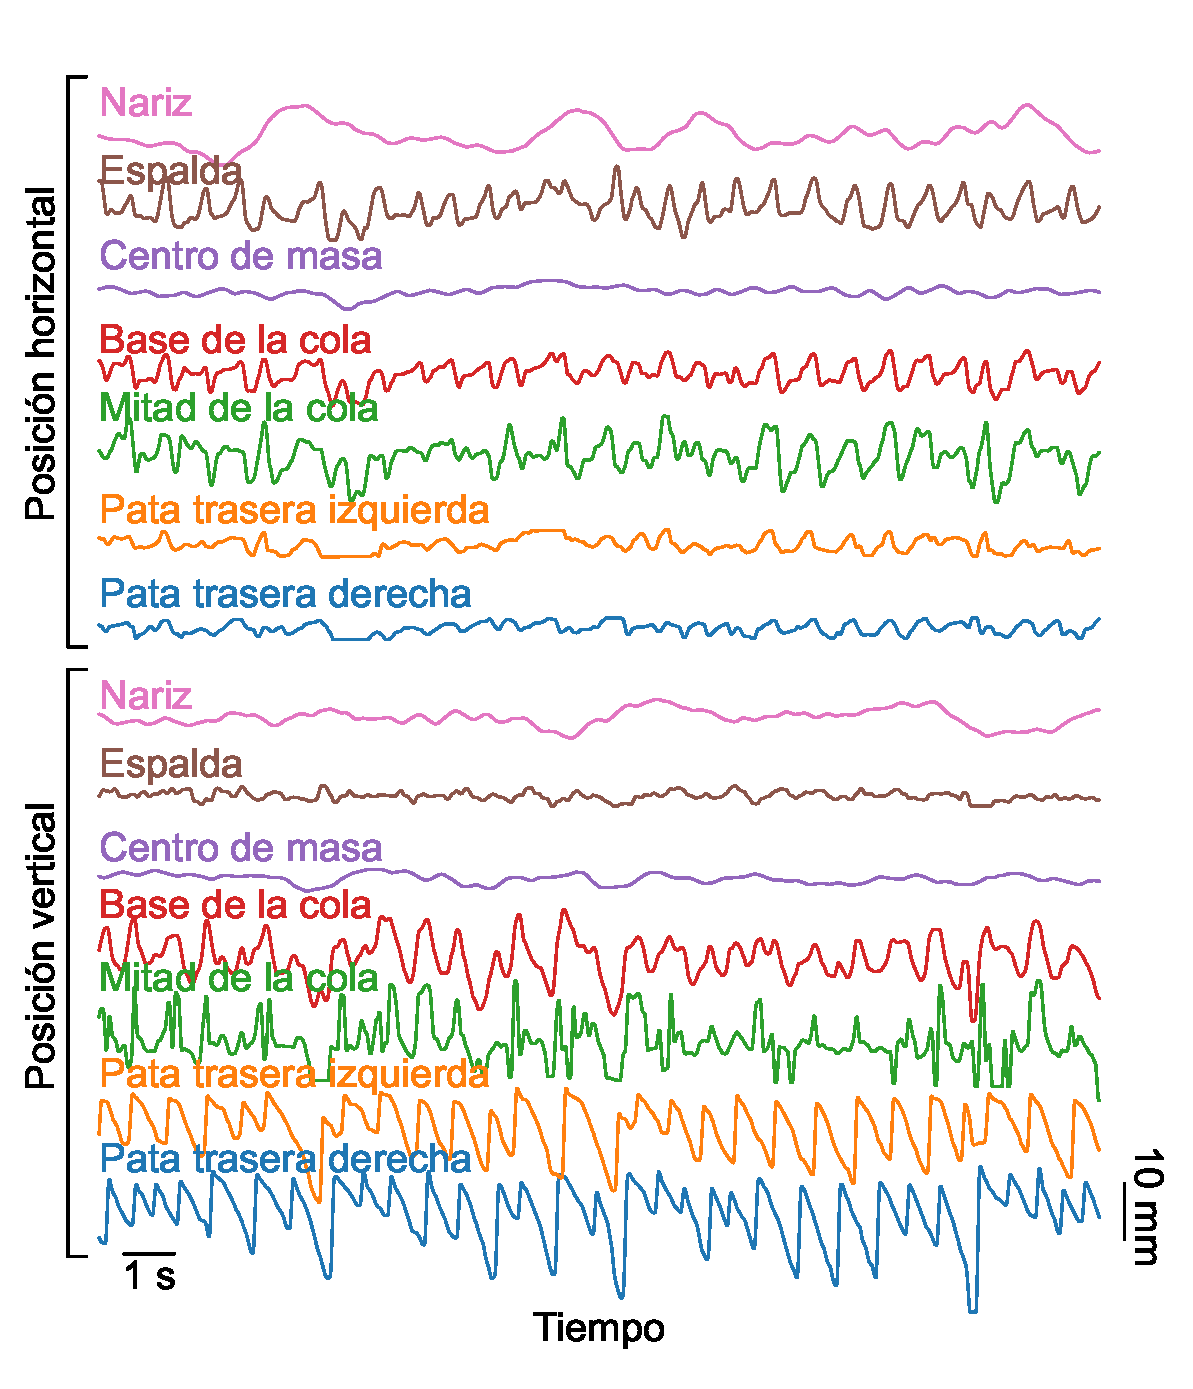
\includegraphics[width=0.6\linewidth]{figuras/capitulo2/posiciones.pdf}
        \caption{\textbf{Posiciones de los marcadores en el tiempo.}
            Seguimiento de marcadores digitales, entre los 75 y 95 s de iniciada una prueba rotarod.
            Se muestran las posiciones horizontales y verticales de los diferentes marcadores en el tiempo.}
        \label{fig:capitulo2_posiciones}
    \end{figure}

    \clearpage

    \section{Ángulos entre partes del cuerpo}\label{sec:apendice_angulos_entre_partes}

    \begin{figure}[htbp]
        \centering
        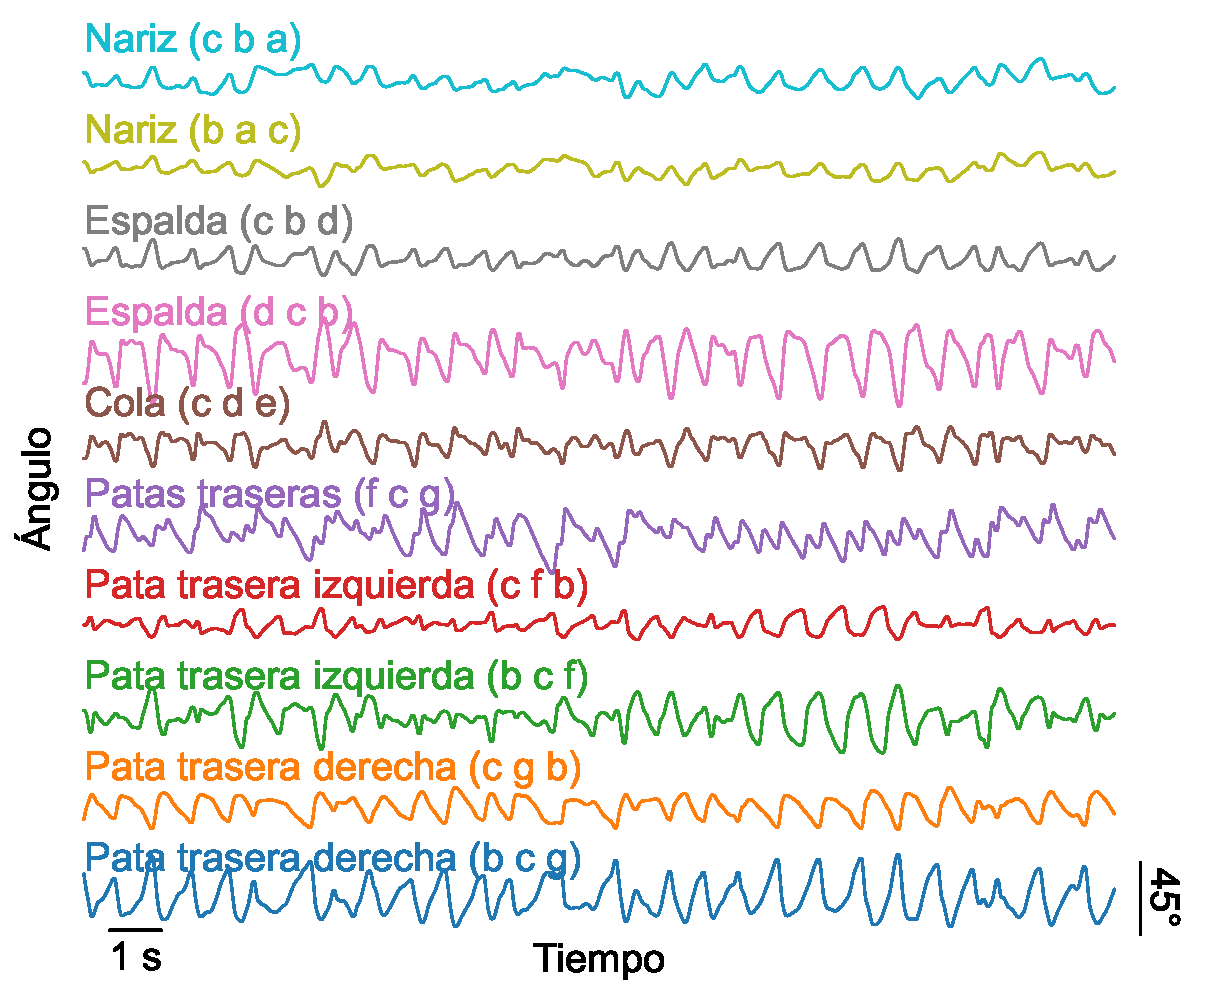
\includegraphics[width=0.6\linewidth]{figuras/capitulo2/angulos.pdf}
        \caption{\textbf{Ángulos de partes del cuerpo en el tiempo.}
            Valores de los ángulos entre los 75 y 95 s de iniciada una prueba rotarod (ídem \autoref{fig:capitulo2_posiciones}).
            Cada ángulo está definido por un triplete (i j k) con i, j, k símbolos de los marcadores.
            Marcadores: (a) nariz, (b) espalda, (c) centro de masa, (d) base de la cola, (e) mitad de la cola, (f) pata trasera izquierda, (g) pata trasera derecha.}
        \label{fig:capitulo2_angulos}
    \end{figure}

    \clearpage

    \section{Espectros \textit{wavelet} y PCA}\label{sec:apendice_pca_wavelet}

    \begin{figure}[htbp]
        \centering
        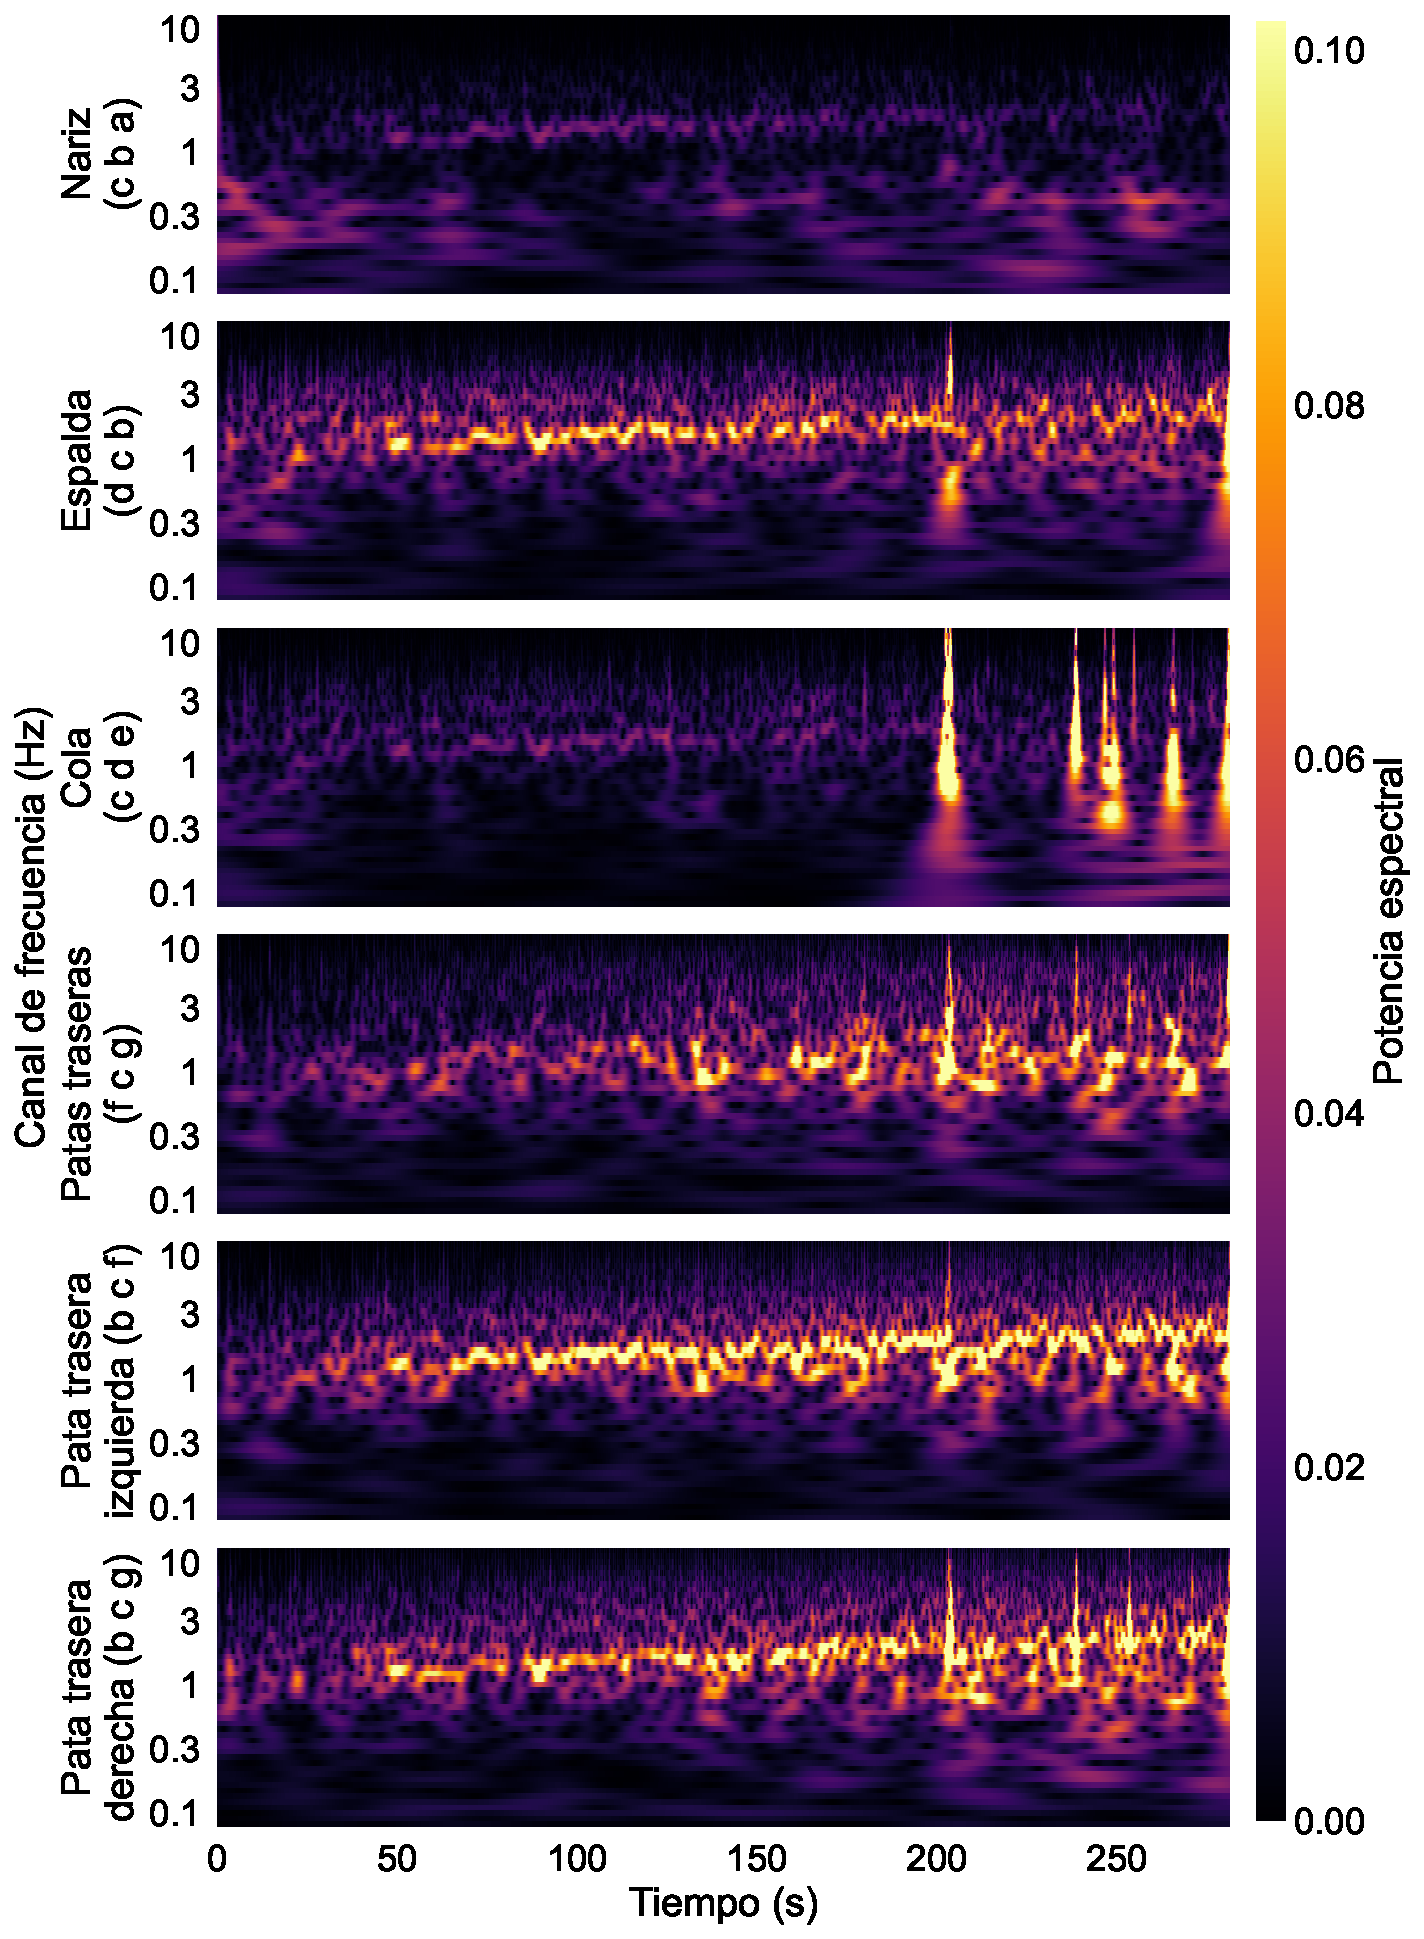
\includegraphics[width=0.7\linewidth]{figuras/capitulo2/espectros_wavelet.pdf}
        \caption{\textbf{Espectros \textit{wavelet} en el tiempo.}
            Espectros de algunos ángulos entre marcadores durante una prueba rotarod (ídem \autoref{fig:capitulo2_posiciones}).
            Cada ángulo está definido por un triplete (i j k) con i, j, k símbolos de los marcadores.
            Marcadores: (a) nariz, (b) espalda, (c) centro de masa, (d) base de la cola, (e) mitad de la cola, (f) pata trasera izquierda, (g) pata trasera derecha.}
        \label{fig:capitulo2_espectros_wavelet}
    \end{figure}

    \begin{figure}[htbp]
        \centering
        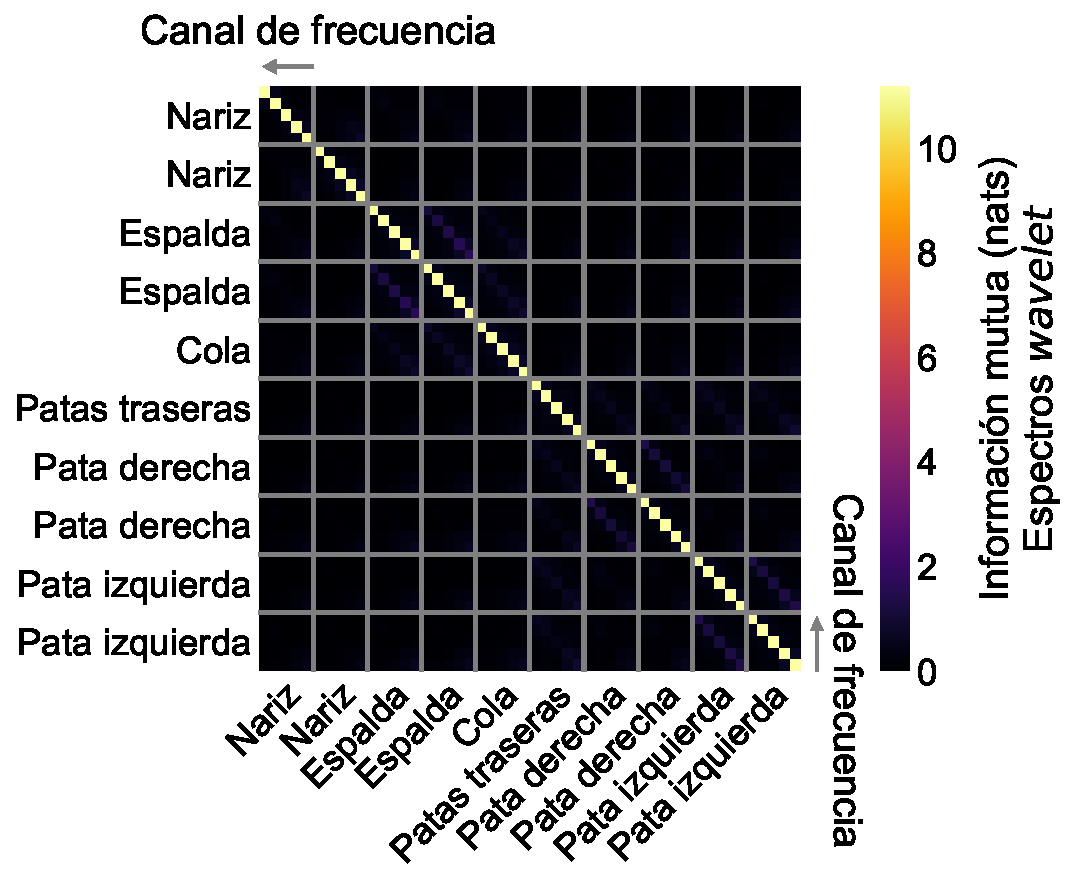
\includegraphics[width=0.7\linewidth]{figuras/capitulo4/mi_mean_wav.pdf}
        \caption{\textbf{Grupos de partes del cuerpo que dependen muy levemente entre sí según sus espectros \textit{wavelet}.}
            Información mutua entre los diferentes canales de frecuencia de los espectros \textit{wavelet} de los ángulos.
            Se observan grupos de ángulos que dependen muy levemente entre sí: patas traseras, espalda-cola y nariz.}
        \label{fig:capitulo2_mi_mean_wav}
    \end{figure}

    \begin{figure}[htbp]
        \centering
        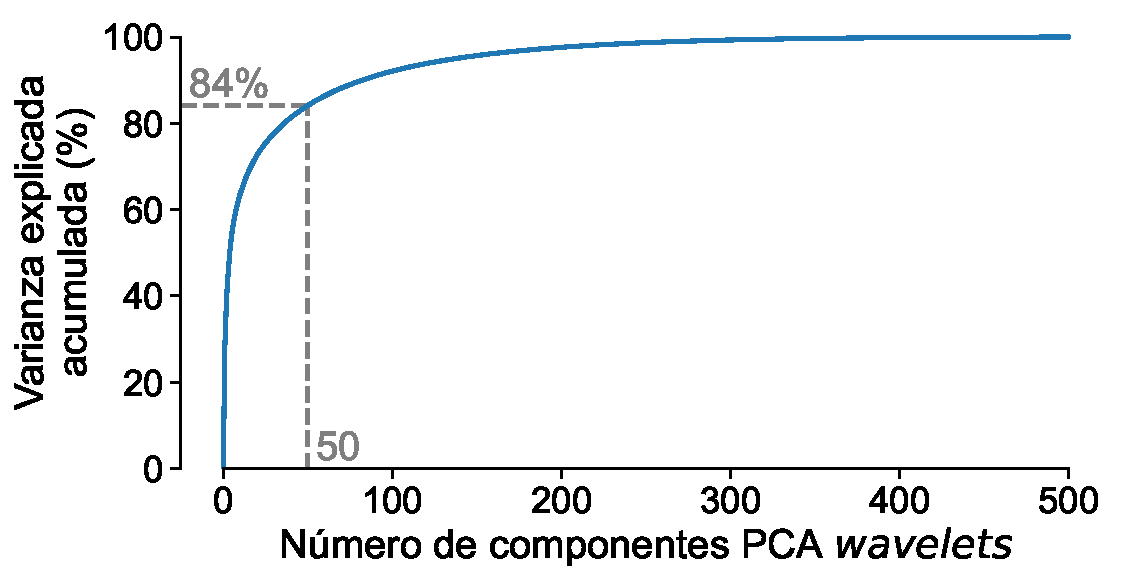
\includegraphics[width=0.7\linewidth]{figuras/capitulo4/varianza_pca.pdf}
        \caption{\textbf{Las 50 primeras componentes principales explican el 84\% de la varianza de los espectros \textit{wavelet}.}
            Varianza explicada acumulada según el número de componentes PCA de los espectros \textit{wavelet}.}
        \label{fig:capitulo4_varianza_pca}
    \end{figure}

    \begin{figure}[htbp]
        \centering
        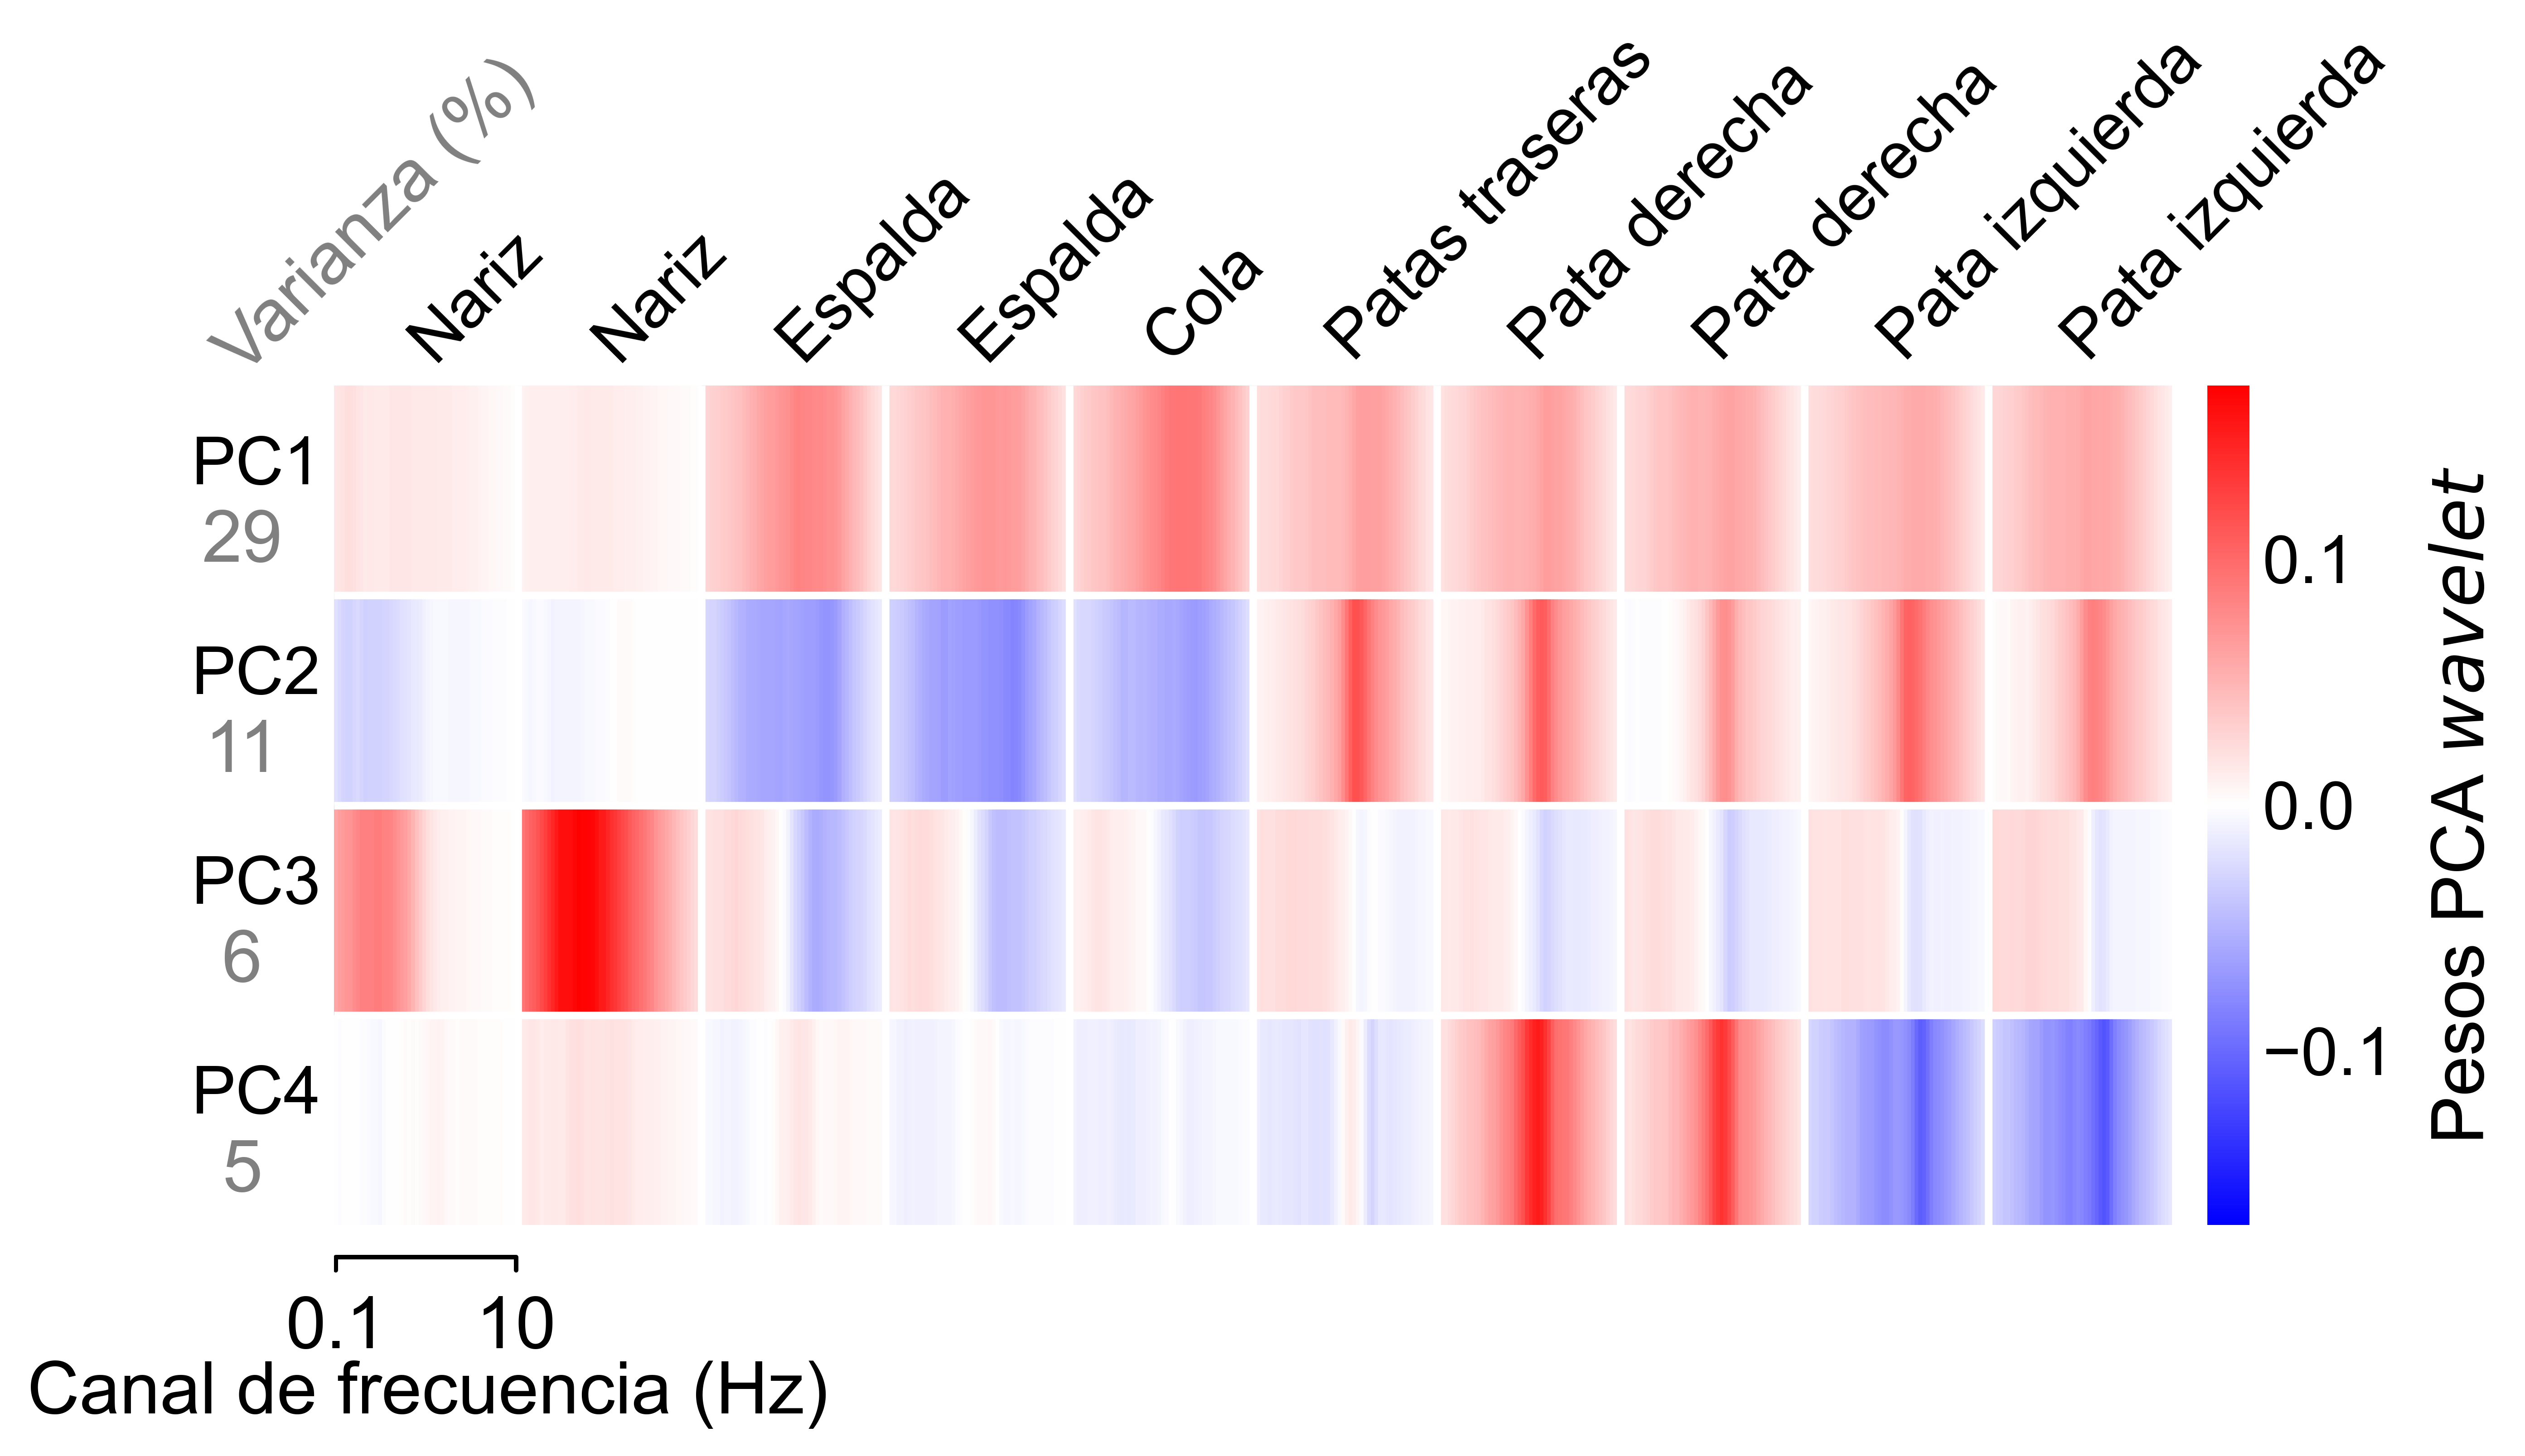
\includegraphics[width=0.8\linewidth]{figuras/capitulo4/pesos_pca.png}
        \caption{\textbf{La primera componente principal de los espectros \textit{wavelet} sigue a la frecuencia espectral promedio.}
            Pesos de las 4 primeras componentes PCA de los espectros \textit{wavelet}, según los canales de frecuencia y las partes del cuerpo involucradas.}
        \label{fig:capitulo4_pesos_pca}
    \end{figure}

    \begin{figure}[htbp]
        \centering
        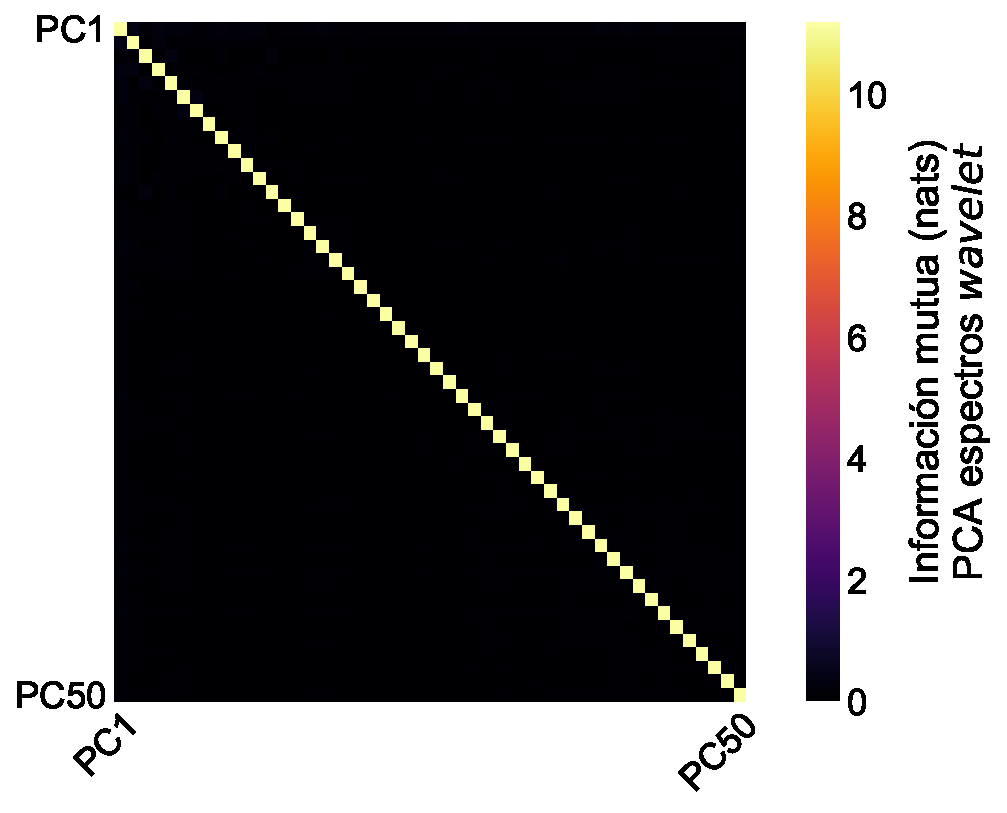
\includegraphics[width=0.7\linewidth]{figuras/capitulo4/mi_pca_wav.pdf}
        \caption{\textbf{Componentes PCA de los espectros \textit{wavelet} son independientes entre sí.}
            Información mutua entre las primeras 50 componentes principales de los espectros \textit{wavelet} de los ángulos.}
        \label{fig:capitulo4_mi_pca_wav}
    \end{figure}

    \begin{figure}[htbp]
        \centering
        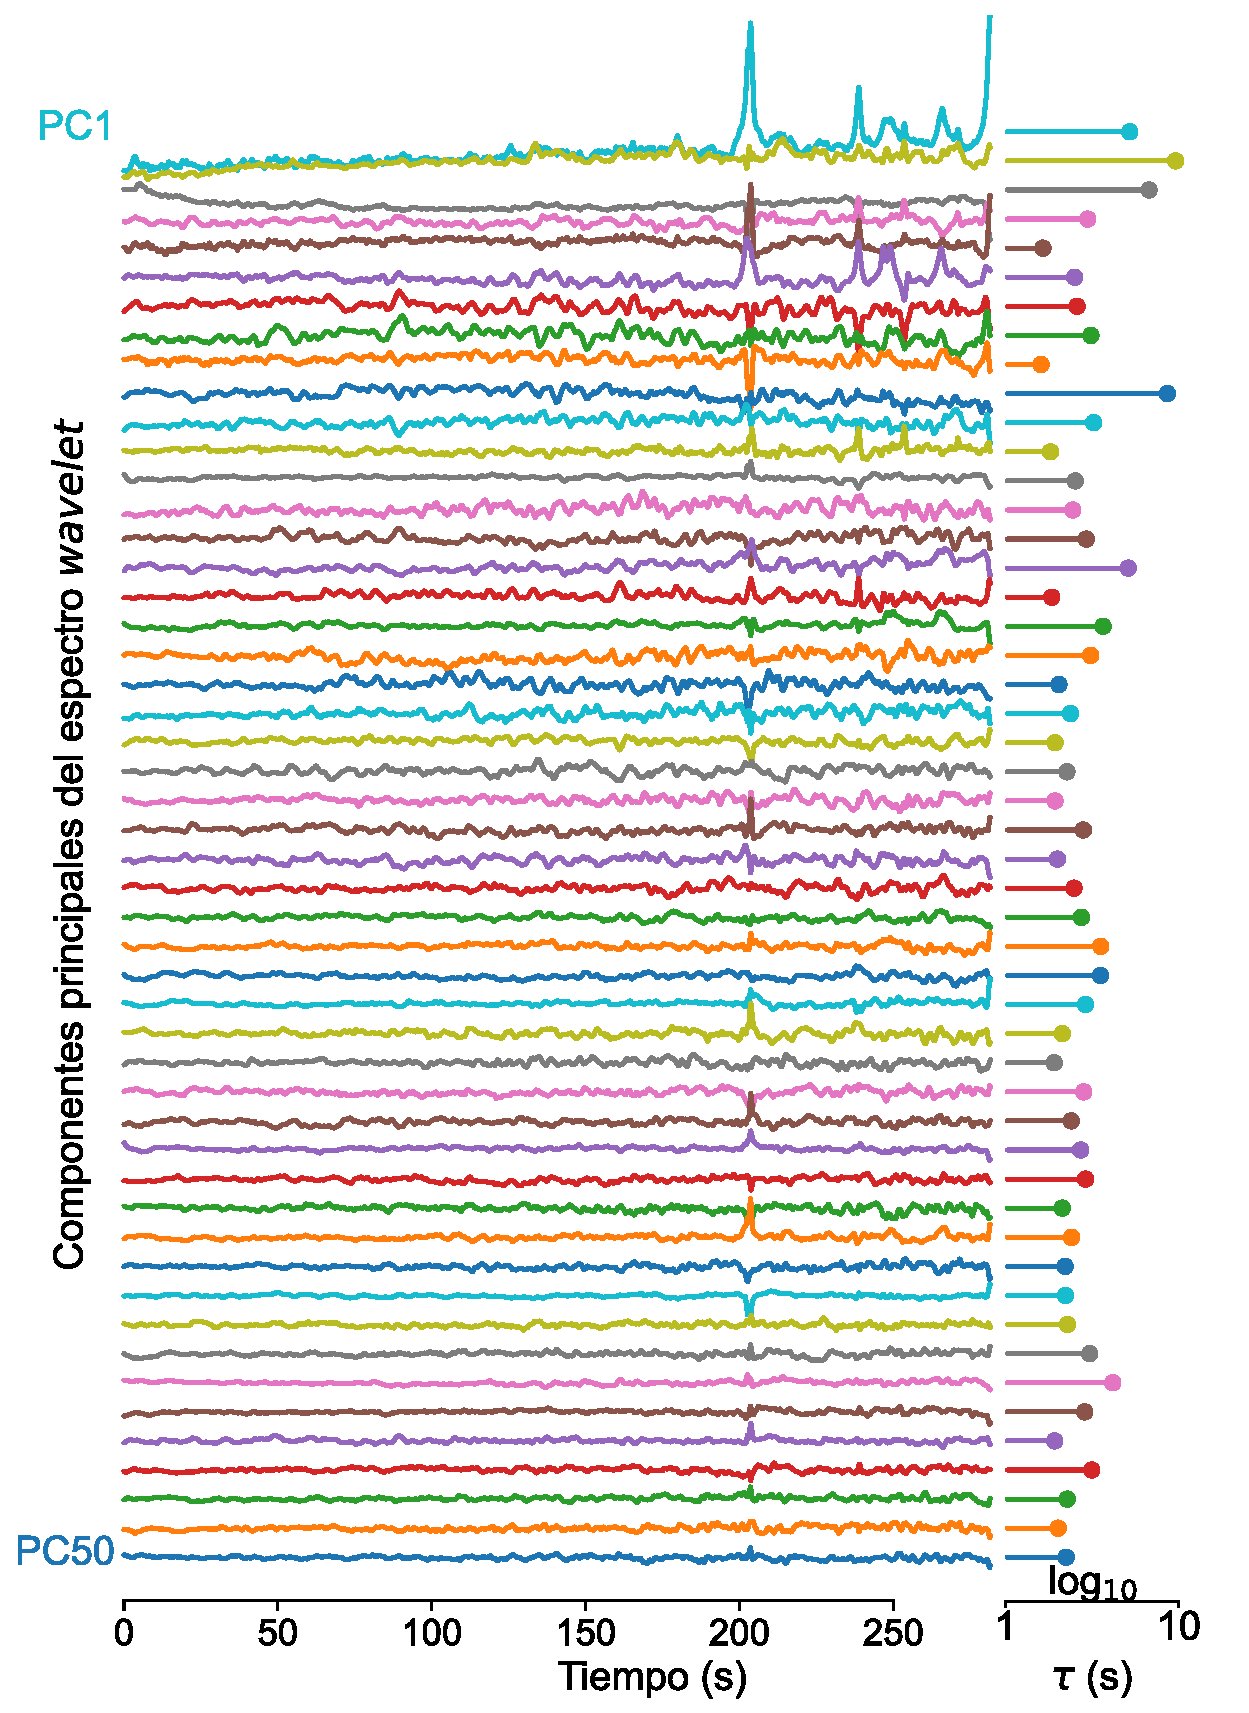
\includegraphics[width=0.7\linewidth]{figuras/capitulo4/componentes_pca.pdf}
        \caption{\textbf{Primeras 50 componentes PCA de los espectros \textit{wavelet}.}
            Ejemplo de los valores que adoptan las primeras 50 componentes PCA de los espectros \textit{wavelet} en una prueba rotarod (ídem \autoref{fig:capitulo2_posiciones}).
            En el margen izquierdo se muestra el tiempo de autocorrelación $\tau$ de cada componente en la prueba.}
        \label{fig:capitulo4_componentes_pca}
    \end{figure}

    \clearpage

    \section{Características de pasos y poses}\label{sec:apendice_pasos_poses}

    \begin{figure}[htbp]
        \centering
        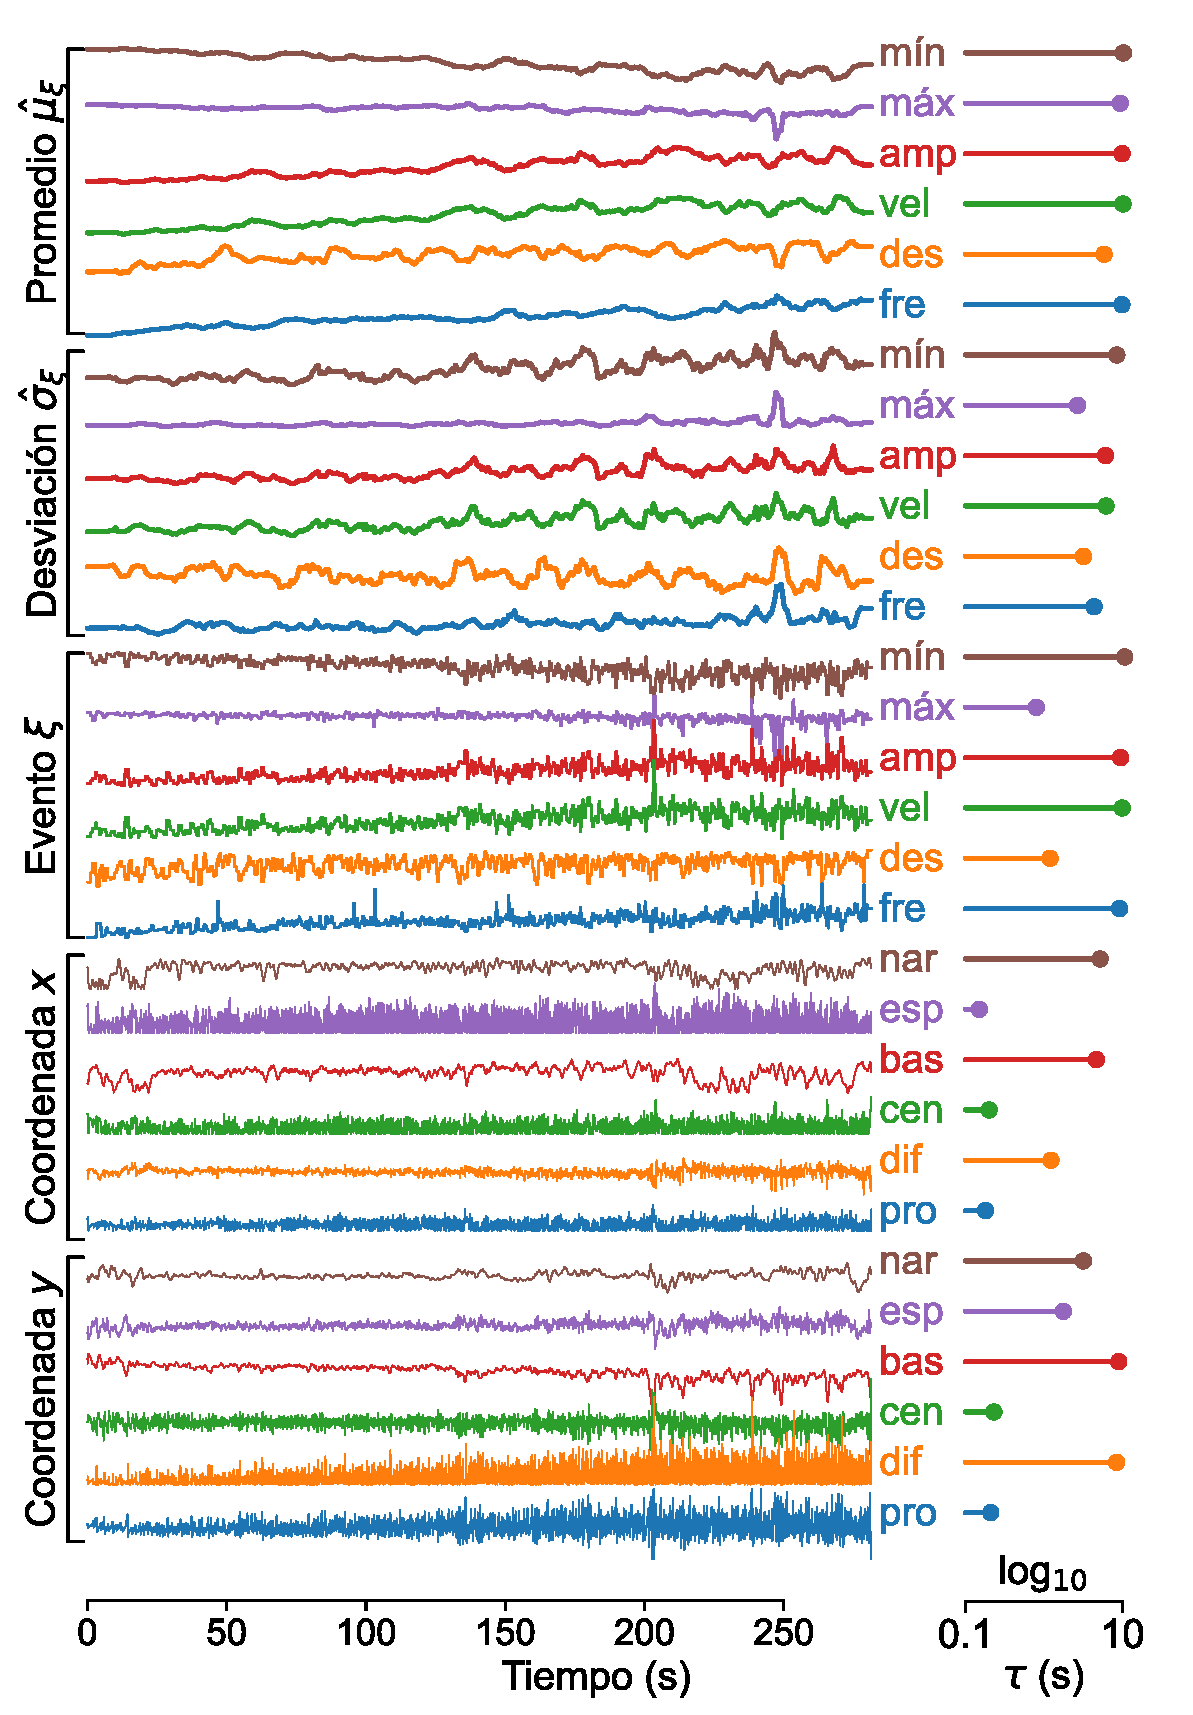
\includegraphics[width=0.7\linewidth]{figuras/capitulo4/caracteristicas_pasos_poses.pdf}
        \caption{\textbf{Características de pasos y poses.}
            Ejemplo de los valores que adoptan las características de pasos y poses en una prueba rotarod (ídem \autoref{fig:capitulo2_posiciones}).
            En el margen izquierdo se muestra el tiempo de autocorrelación $\tau$ de cada característica en la prueba.
            Abreviaturas: (min) altura mínima, (max) altura máxima, (amp) amplitud, (vel) velocidad, (des) desfasaje, (fre) frecuencia,
            (nar) nariz, (esp) espalda, (bas) base de la cola, (cen) centro de masa, (dif) diferencia entre patas traseras, (pro) promedio entre patas traseras.}
        \label{fig:capitulo4_caracteristicas_pasos_poses}
    \end{figure}

    \begin{figure}[htbp]
        \centering
        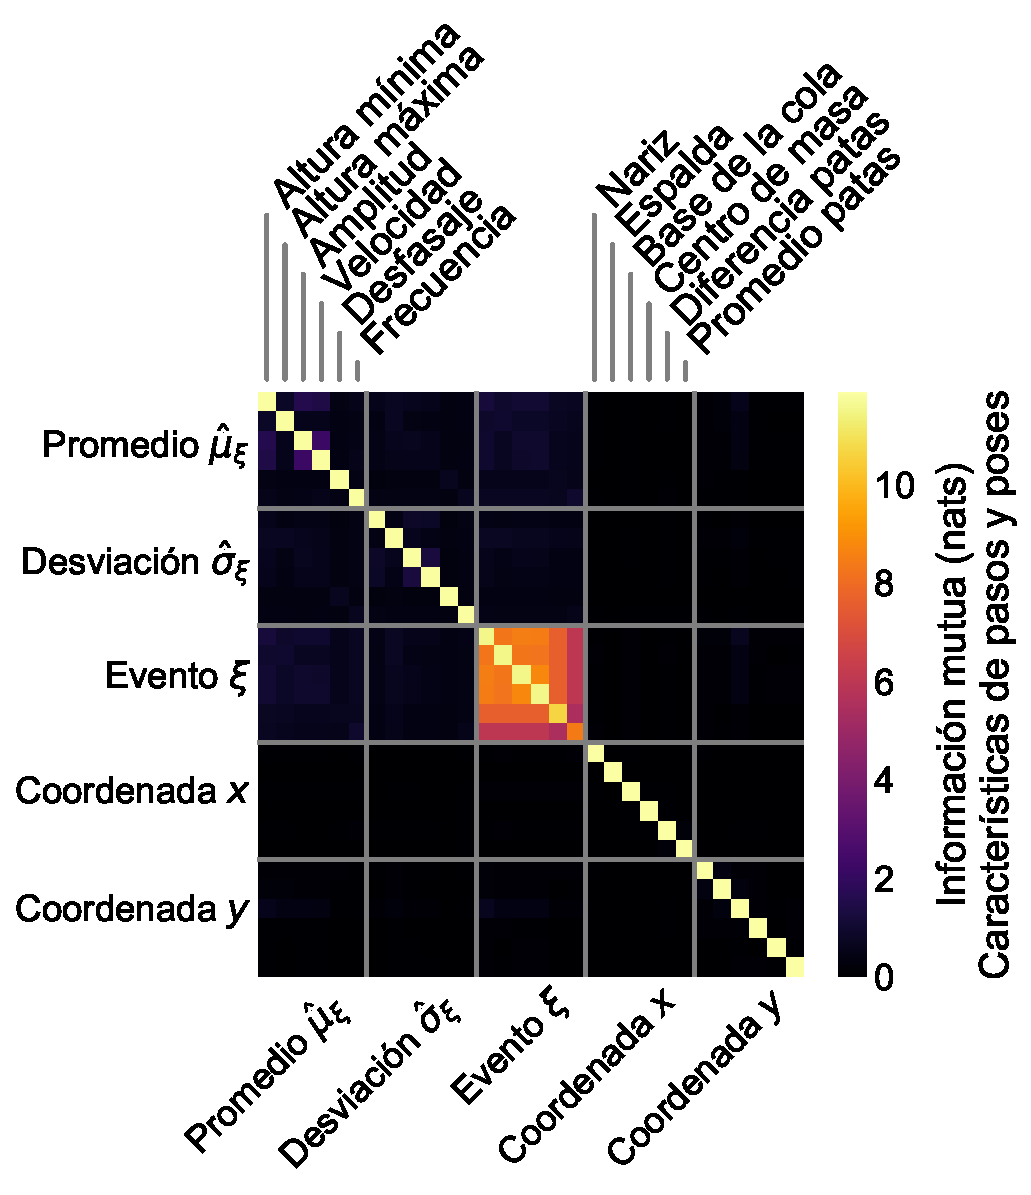
\includegraphics[width=0.7\linewidth]{figuras/capitulo4/mi_scaler_stp.pdf}
        \caption{\textbf{Características de pasos dependen más fuertemente entre sí en los eventos.}
            Información mutua entre las diferentes las diferentes variables de las características de los pasos y poses.}
        \label{fig:capitulo4_mi_scaler_stp}
    \end{figure}

    \begin{figure}[htbp]
        \centering
        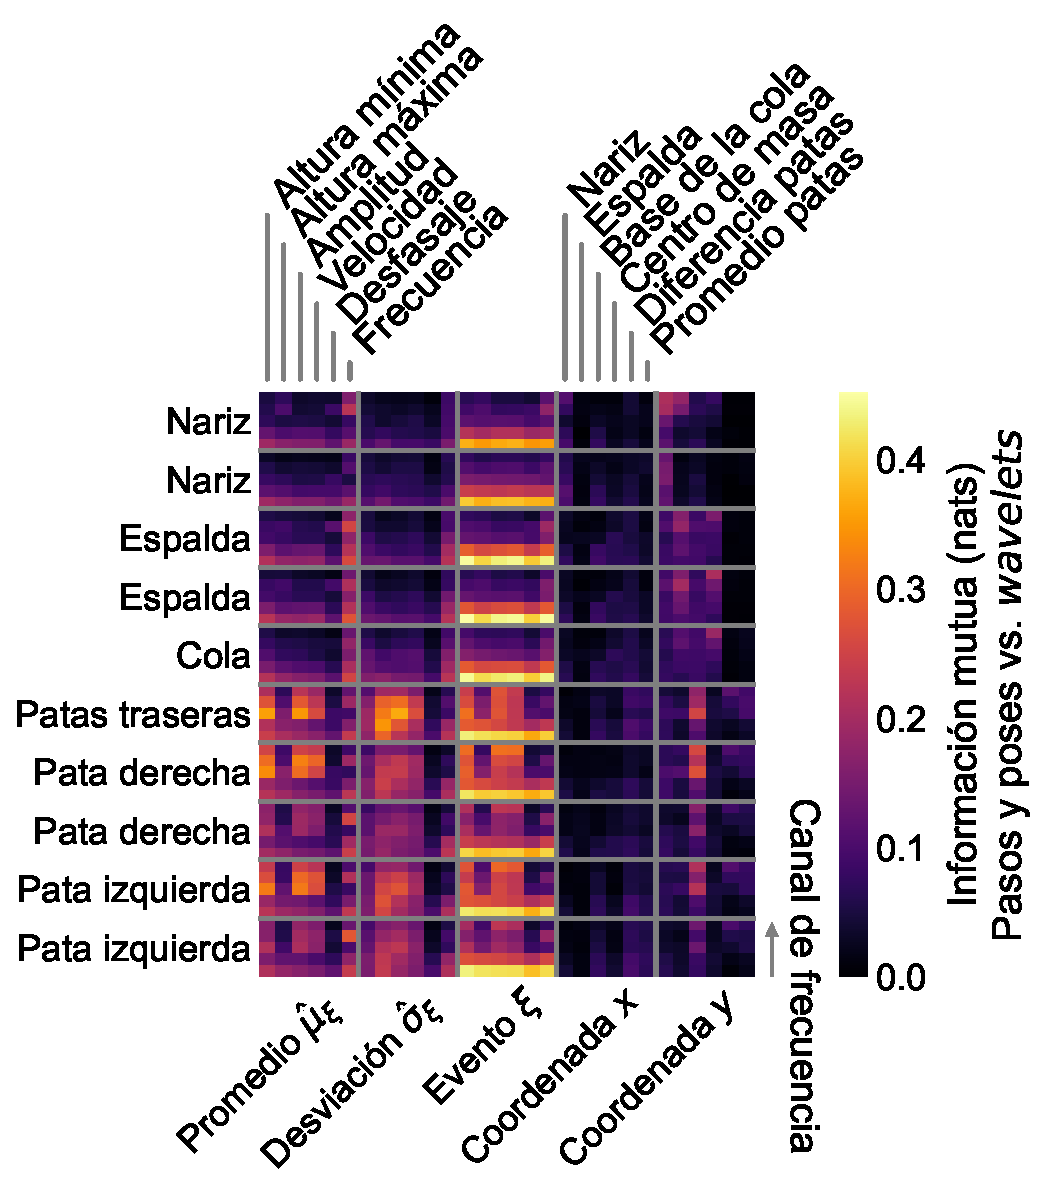
\includegraphics[width=0.75\linewidth]{figuras/capitulo4/mi_mean_wav_scaler_stp.pdf}
        \caption{\textbf{Información mutua pasos y poses vs. espectros \textit{wavelet}.}}
        \label{fig:capitulo4_mi_mean_wav_scaler_stp}
    \end{figure}

    \begin{figure}[htbp]
        \centering
        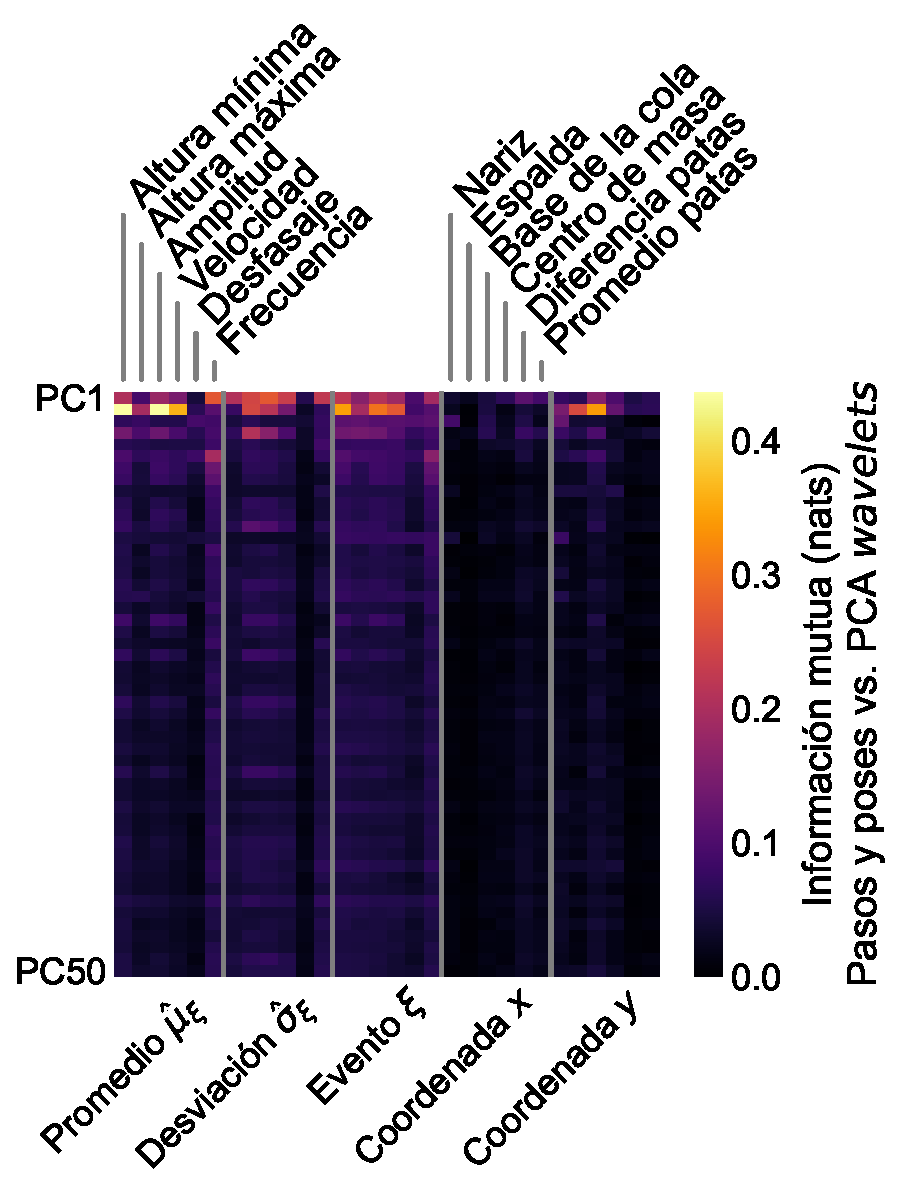
\includegraphics[width=0.7\linewidth]{figuras/capitulo4/mi_pca_wav_scaler_stp.pdf}
        \caption{\textbf{Información mutua pasos y poses vs. PCA \textit{wavelets}.}}
        \label{fig:capitulo4_mi_pca_wav_scaler_stp}
    \end{figure}

    \clearpage

    \chapter{Métricas de comportamiento}\label{cha:apendice_metricas}

    Figuras suplementarias acerca de la evolución de las diferentes métricas comportamentales calculadas a partir de las características de pasos durante los primeros 100 s de la ejecución de las pruebas rotarod.

    \clearpage

    \section{Promedio}\label{sec:apendice_promedio}

    \begin{figure}[htbp]
        \centering
        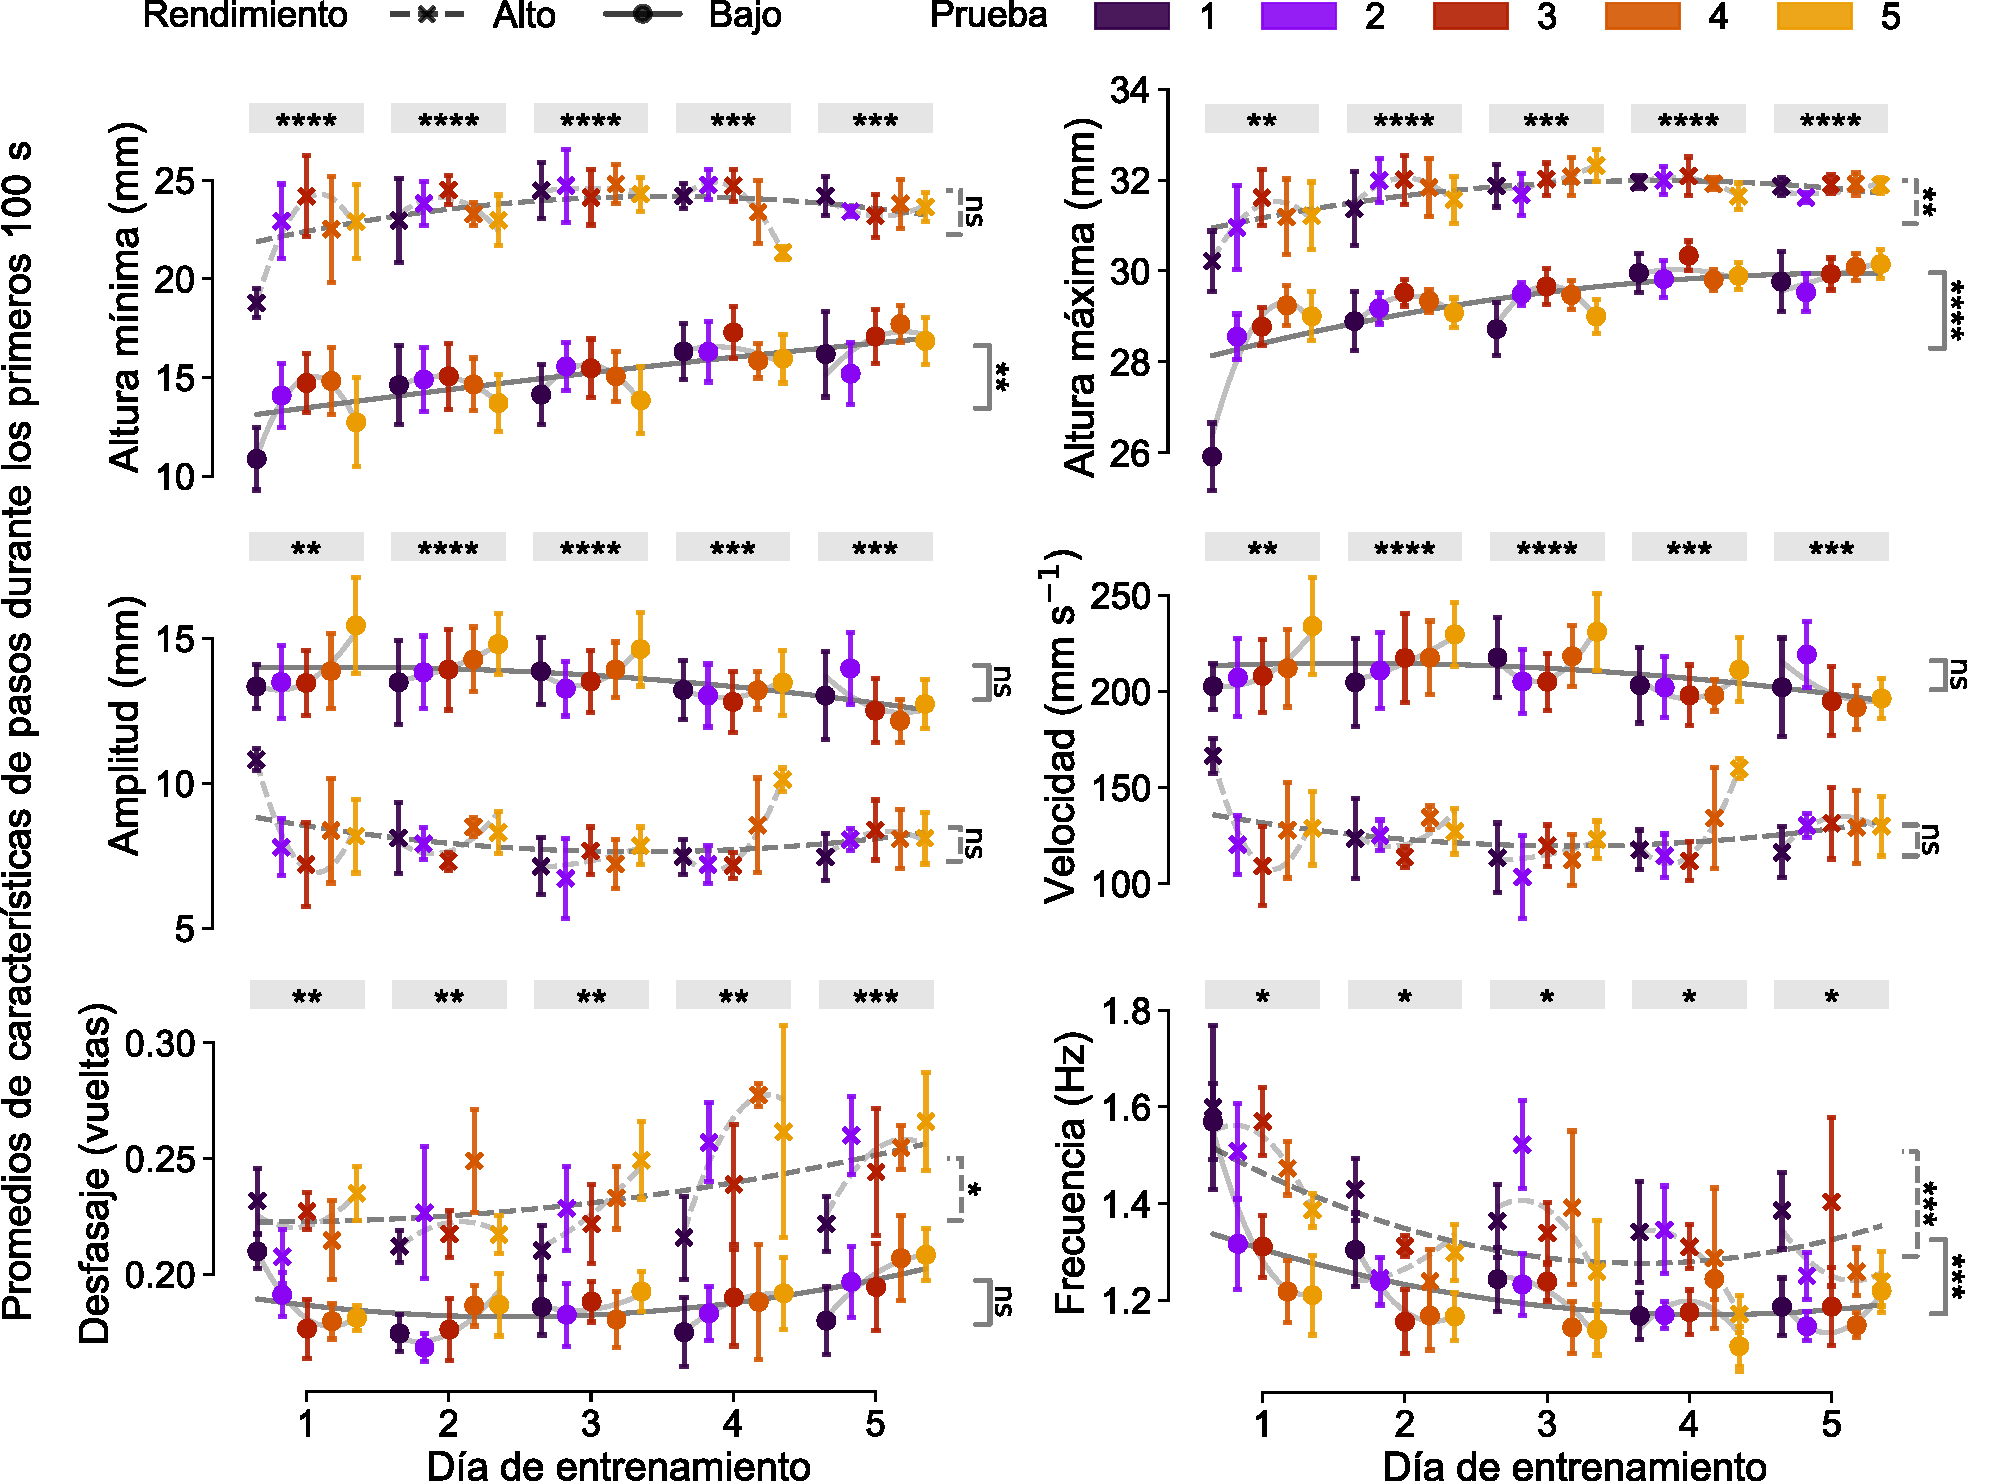
\includegraphics[width=0.99\linewidth]{figuras/capitulo3/metricas_promedio.pdf}
        \caption{\textbf{Promedio de las características de pasos durante los primeros 100 s de las pruebas rotarod.} Los puntos muestran el promedio por grupo de rendimiento y las barras son el error estándar del promedio.
            En cada subfigura, los rectángulos grises superiores indican los p-valores T-test entre grupos de rendimiento para cada día.
            Los corchetes en los márgenes derechos indican, para cada grupo de rendimiento, los p-valores \textit{one-way} ANOVA agrupando por día de entrenamiento.}
        \label{fig:capitulo3_metricas_promedio}
    \end{figure}

    \clearpage

    \section{Pendiente}\label{sec:apendice_pendiente}

    \begin{figure}[htbp]
        \centering
        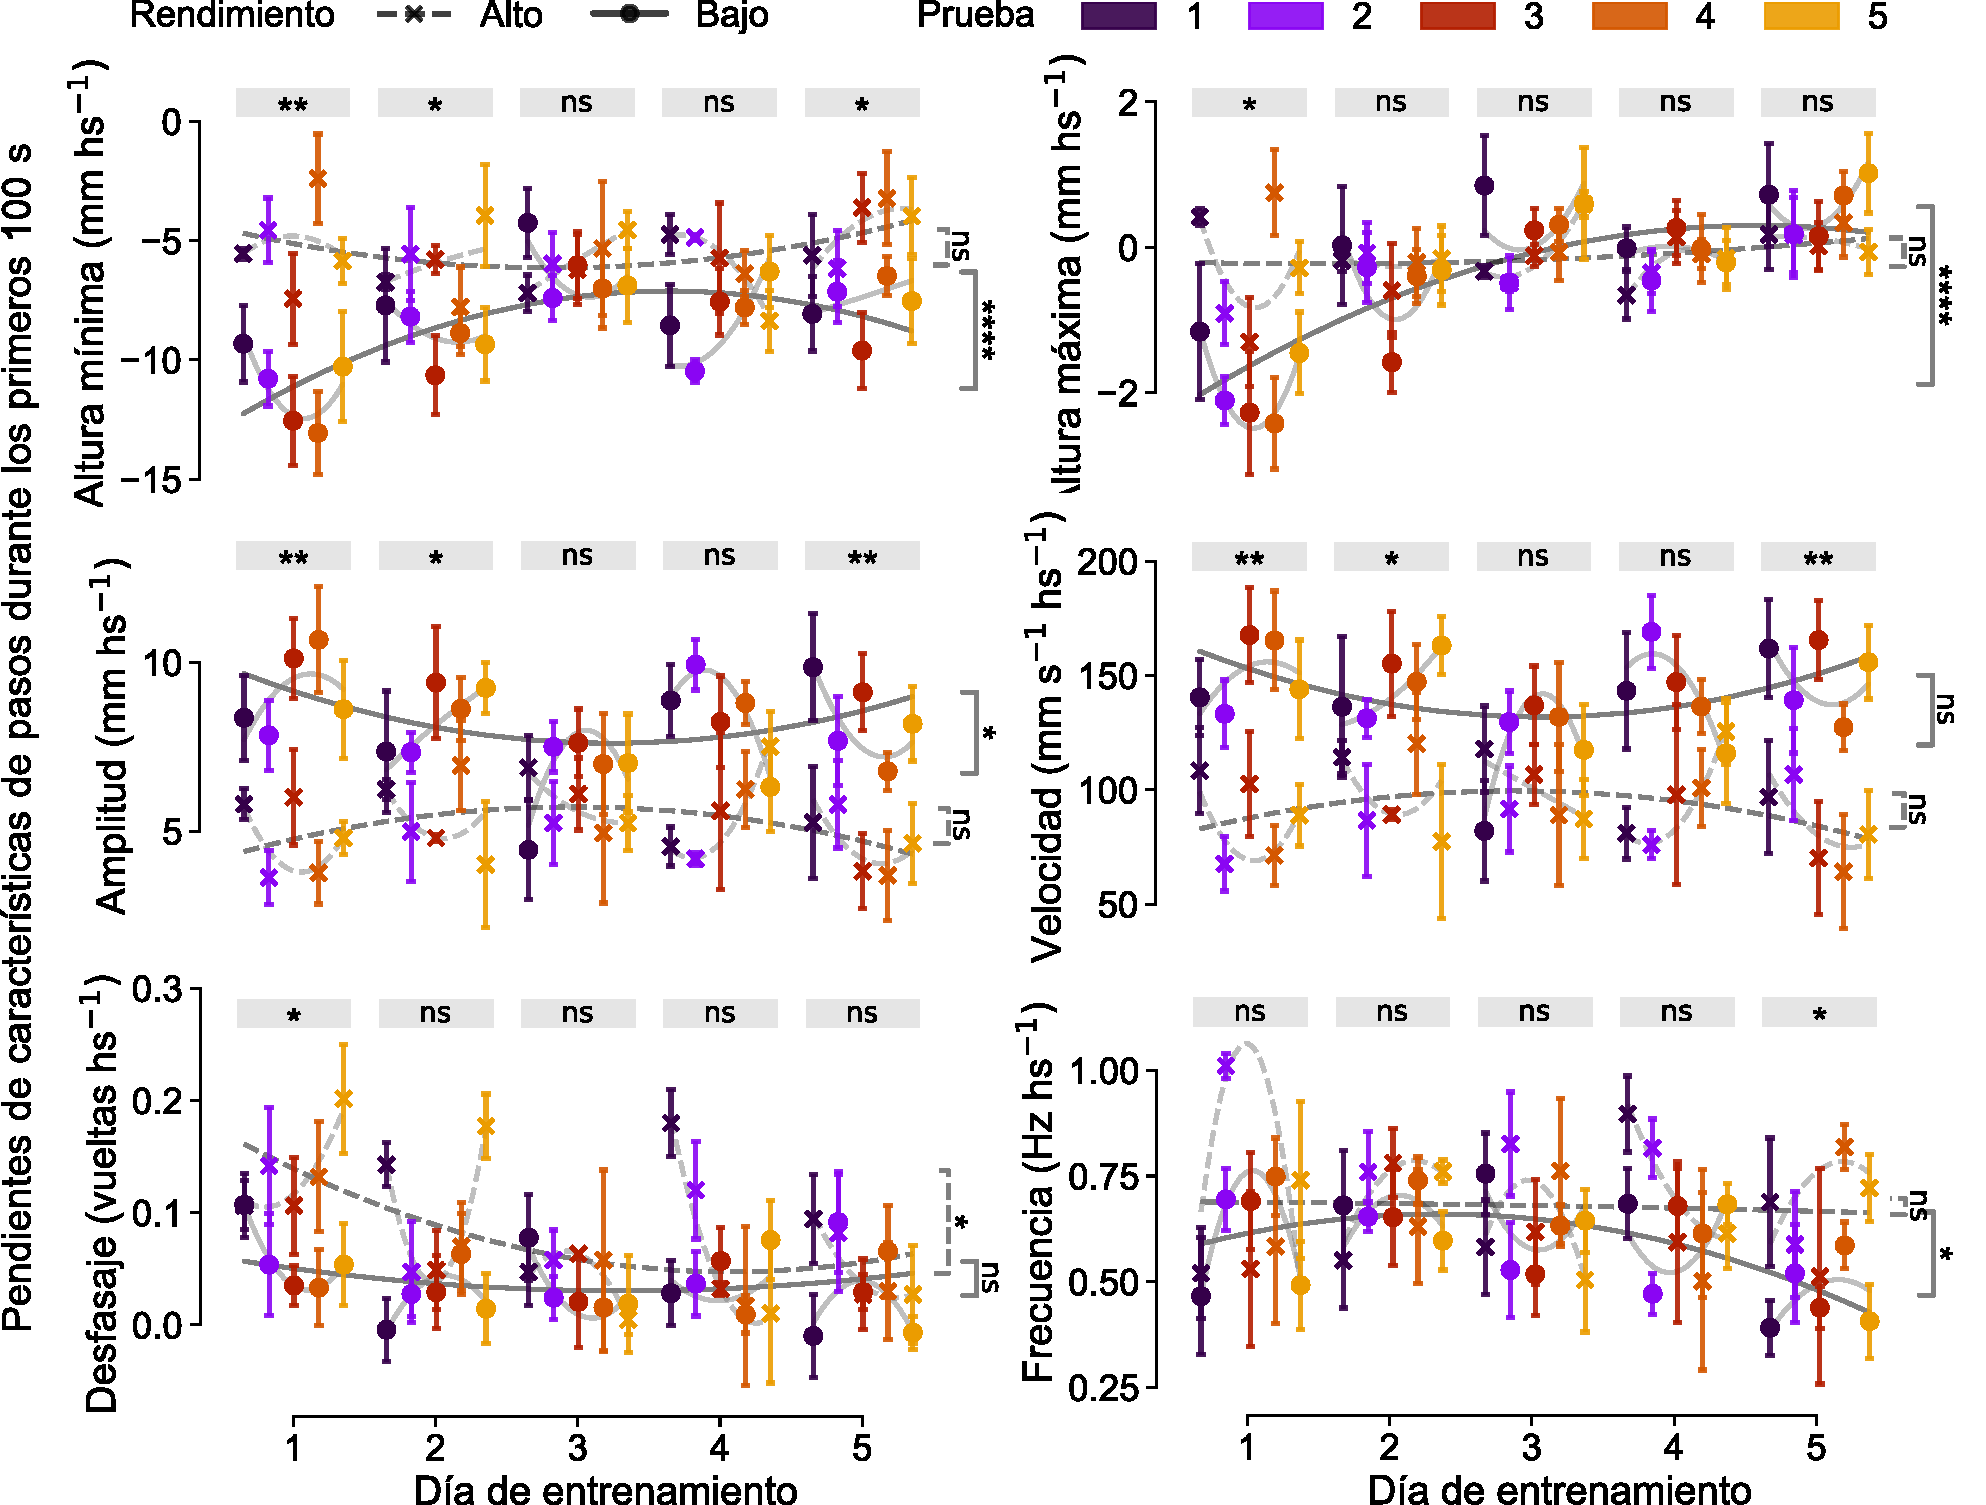
\includegraphics[width=0.99\linewidth]{figuras/capitulo3/metricas_pendiente.pdf}
        \caption{\textbf{Pendiente de las características de pasos durante los primeros 100 s de las pruebas rotarod.} Los puntos muestran el promedio por grupo de rendimiento y las barras son el error estándar del promedio.
            En cada subfigura, los rectángulos grises superiores indican los p-valores T-test entre grupos de rendimiento para cada día.
            Los corchetes en los márgenes derechos indican, para cada grupo de rendimiento, los p-valores \textit{one-way} ANOVA agrupando por día de entrenamiento.}
        \label{fig:capitulo3_metricas_pendiente}
    \end{figure}

    \clearpage

    \section{RMSE}\label{sec:apendice_rmse}

    \begin{figure}[htbp]
        \centering
        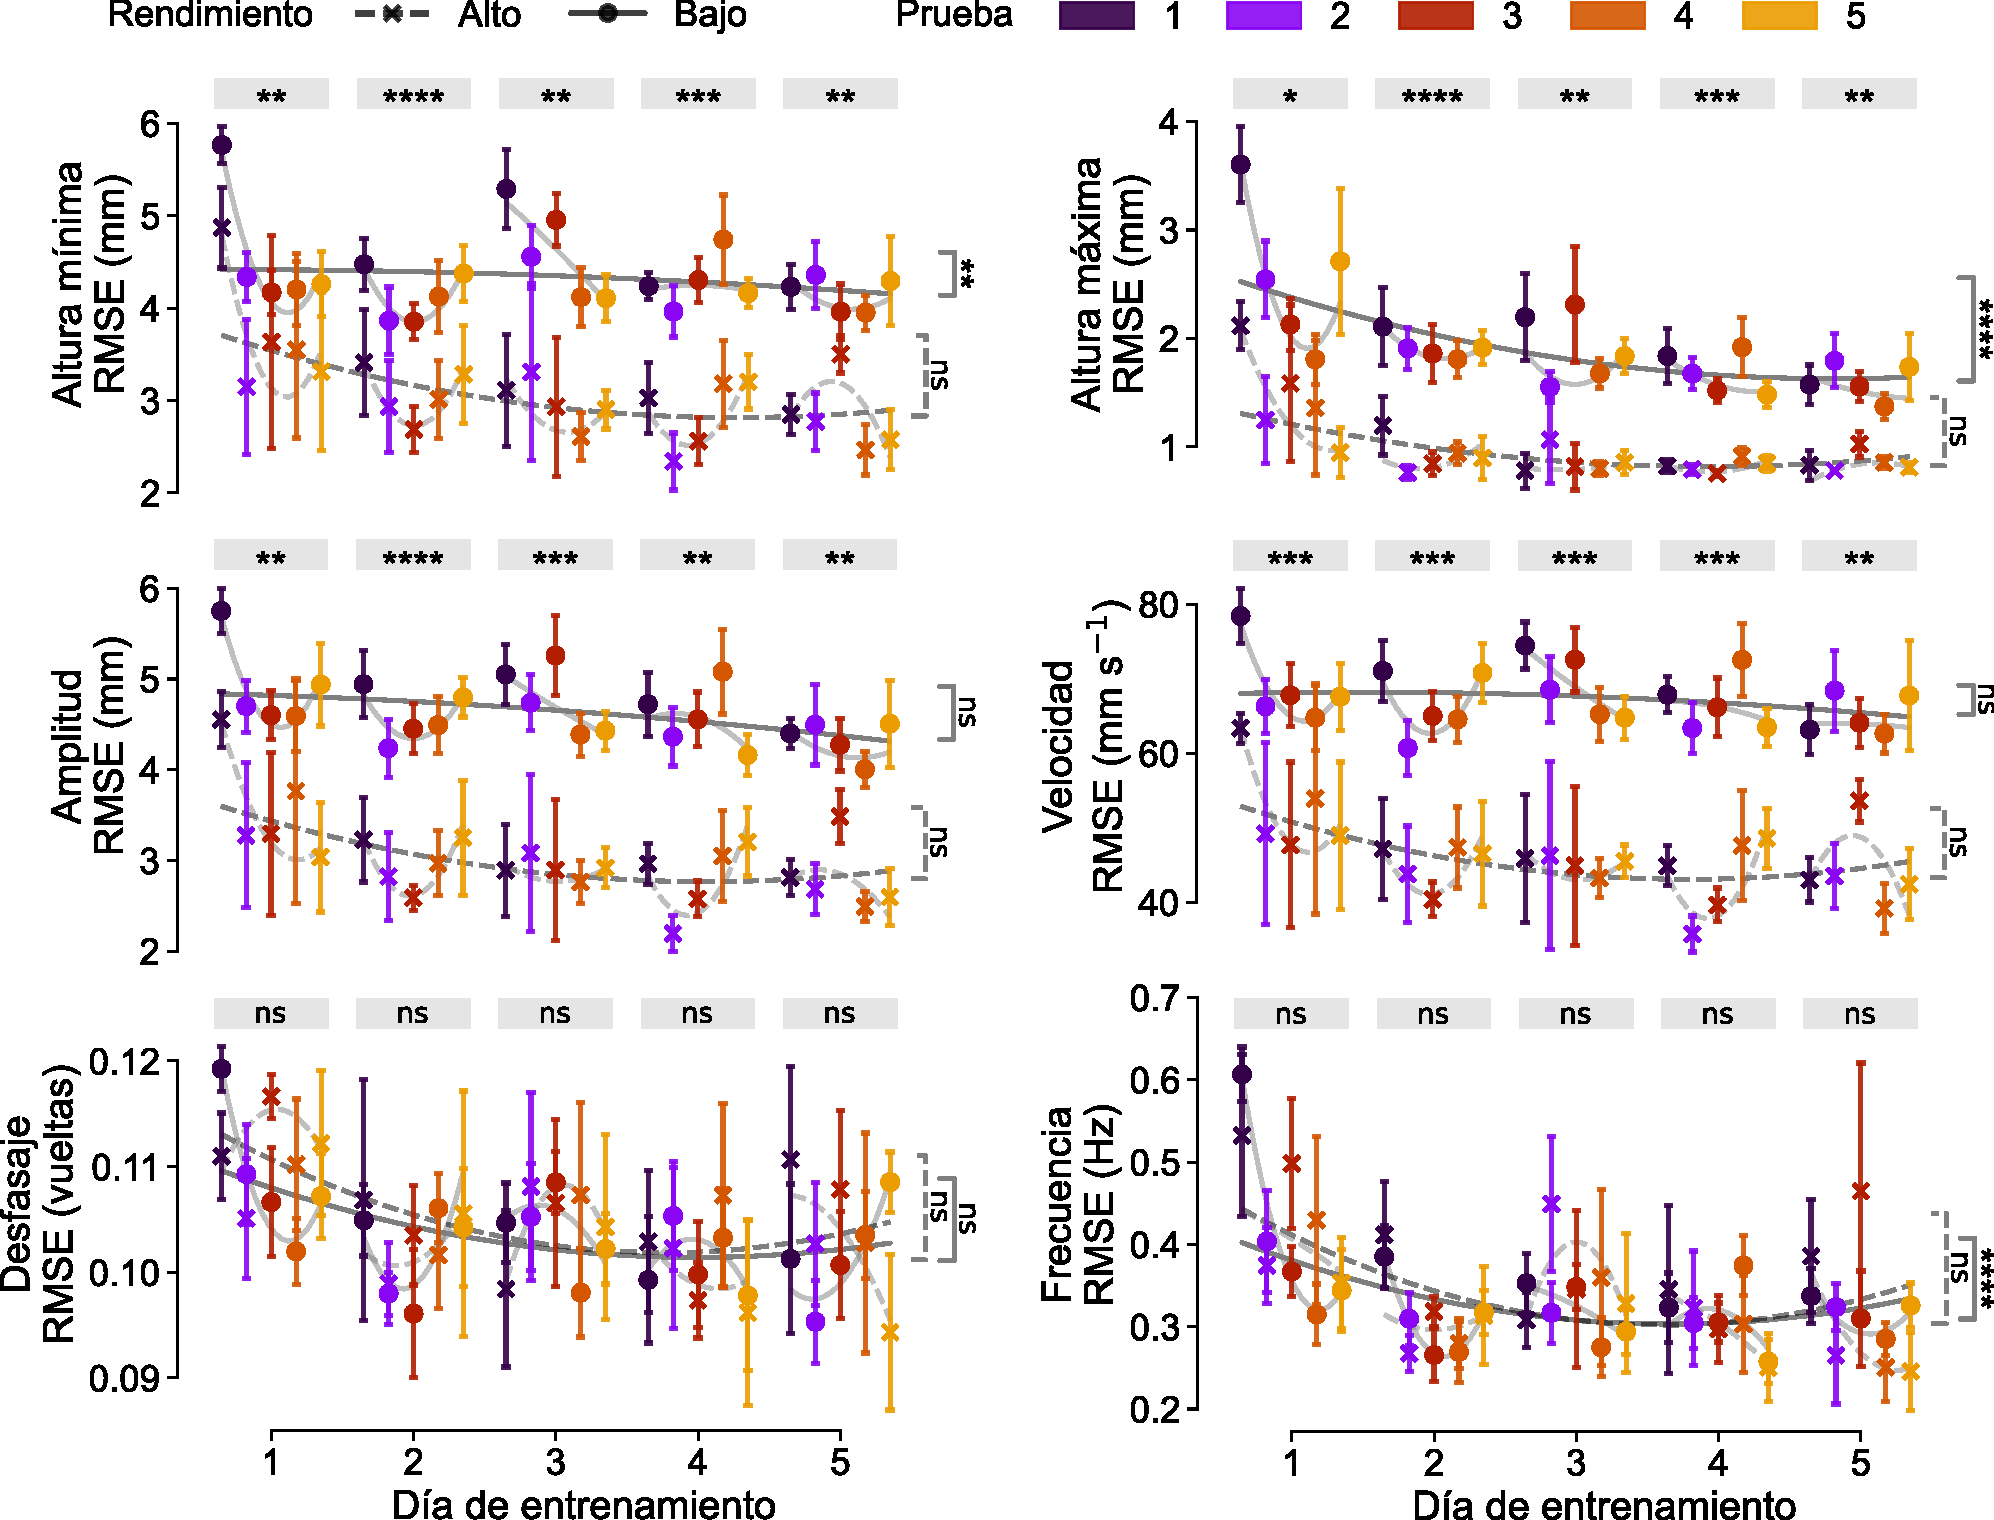
\includegraphics[width=0.99\linewidth]{figuras/capitulo3/metricas_rmse.pdf}
        \caption{\textbf{RMSE de las características de pasos durante los primeros 100 s de las pruebas rotarod.} Los puntos muestran el promedio por grupo de rendimiento y las barras son el error estándar del promedio.
            En cada subfigura, los rectángulos grises superiores indican los p-valores T-test entre grupos de rendimiento para cada día.
            Los corchetes en los márgenes derechos indican, para cada grupo de rendimiento, los p-valores \textit{one-way} ANOVA agrupando por día de entrenamiento.}
        \label{fig:capitulo3_metricas_rmse}
    \end{figure}

    \clearpage

    \chapter{Análisis de mapas de comportamiento}\label{cha:apendice_mapas}

    Figuras suplementarias sobre el análisis de las proyecciones UMAP y los \textit{labels} de comportamiento obtenidos a partir de los dos conjuntos de características: PCA de los espectros \textit{wavelet} y características de pasos y poses.

    \section{Caracterización de los mapas UMAP}\label{sec:apendice_umap}

    \begin{figure}[htbp]
        \centering
        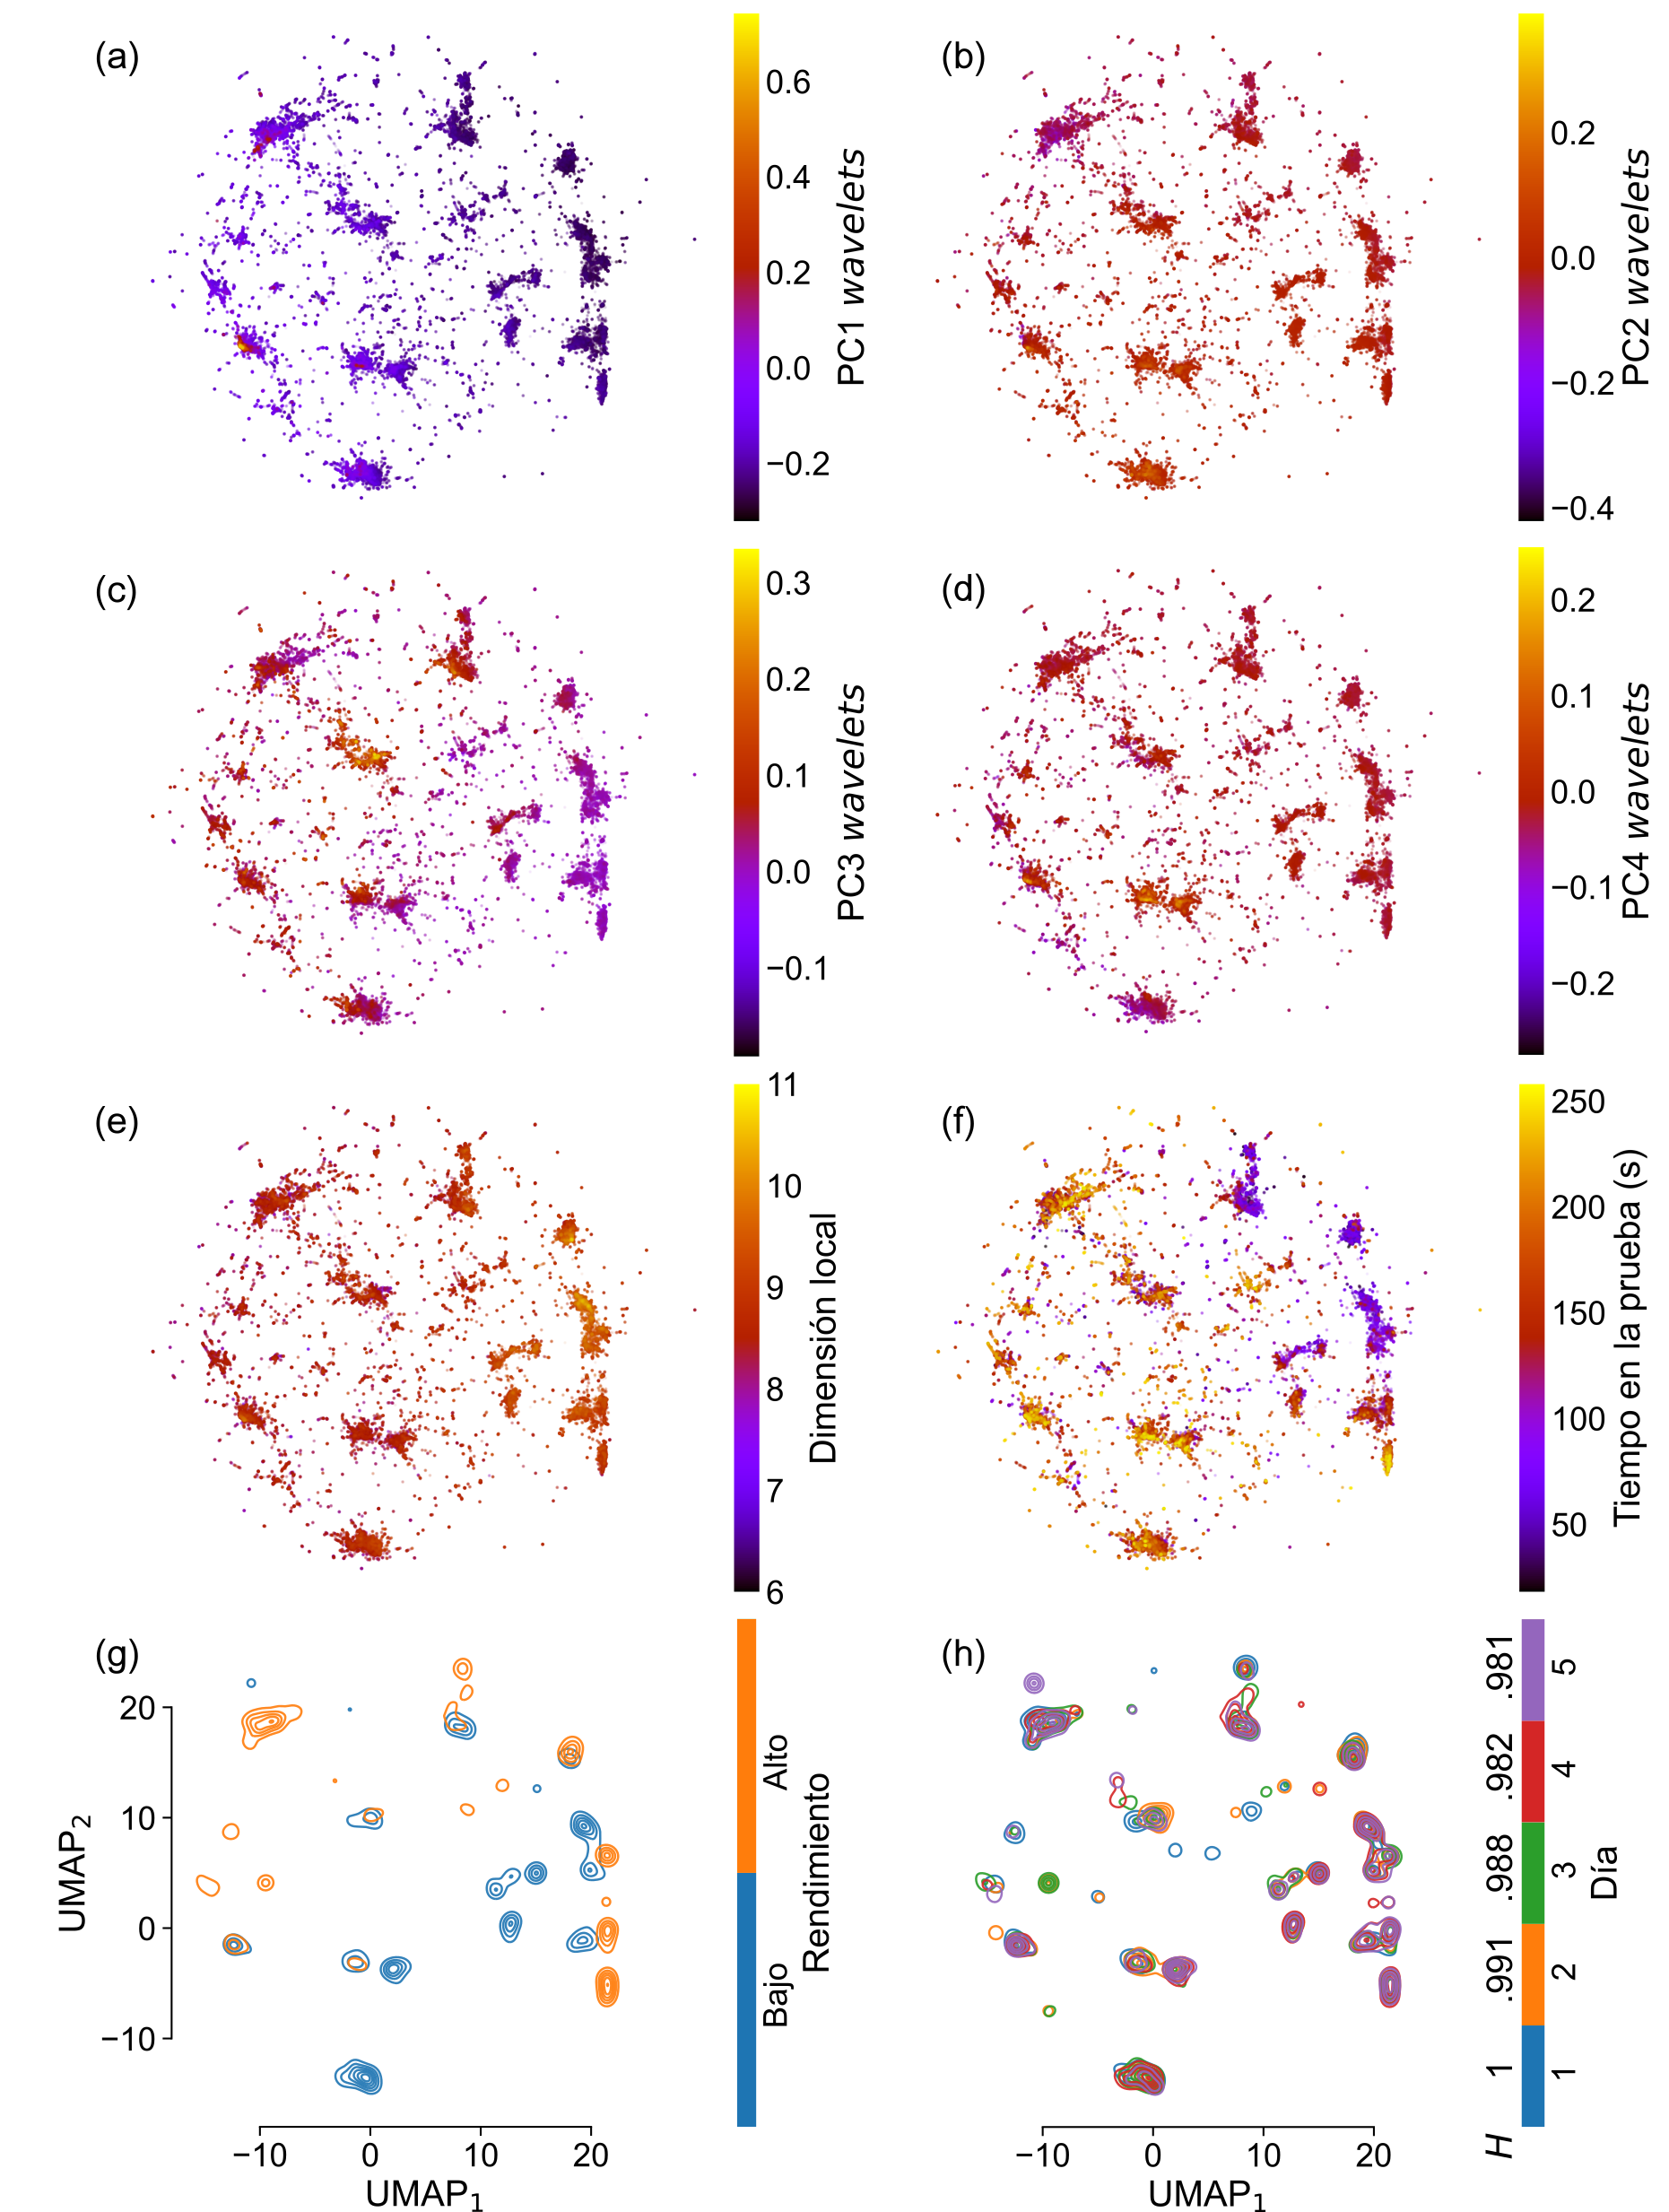
\includegraphics[width=0.9\linewidth]{figuras/capitulo4/umap_wav.png}
        \caption{\textbf{UMAP de las componentes principales de los espectros \textit{wavelet}.} Valores de las primeras cuatro componentes principales (PCs): (a) PC1, (b) PC2, (c) PC3 y (d) PC4. (e) Dimensión local del mapa. La dimensión local es el número de componentes PCA que explican el 80\% de la varianza en el subconjunto de datos formado por los vecinos más cercanos de cada punto en el mapa. (f) Tiempo transcurrido en cada prueba rotarod. (g) Densidad de probabilidad  en el espacio UMAP, condicionada por grupo de rendimiento. (h) Densidad de probabilida condicionada por día de entrenamiento. La entropía $H$ de las distribuciones disminuye con los días de entrenamiento, tomando como valor de referencia a la entropía del día 1.}
        \label{fig:capitulo4_umap_wav}
    \end{figure}

    \begin{figure}[htbp]
        \centering
        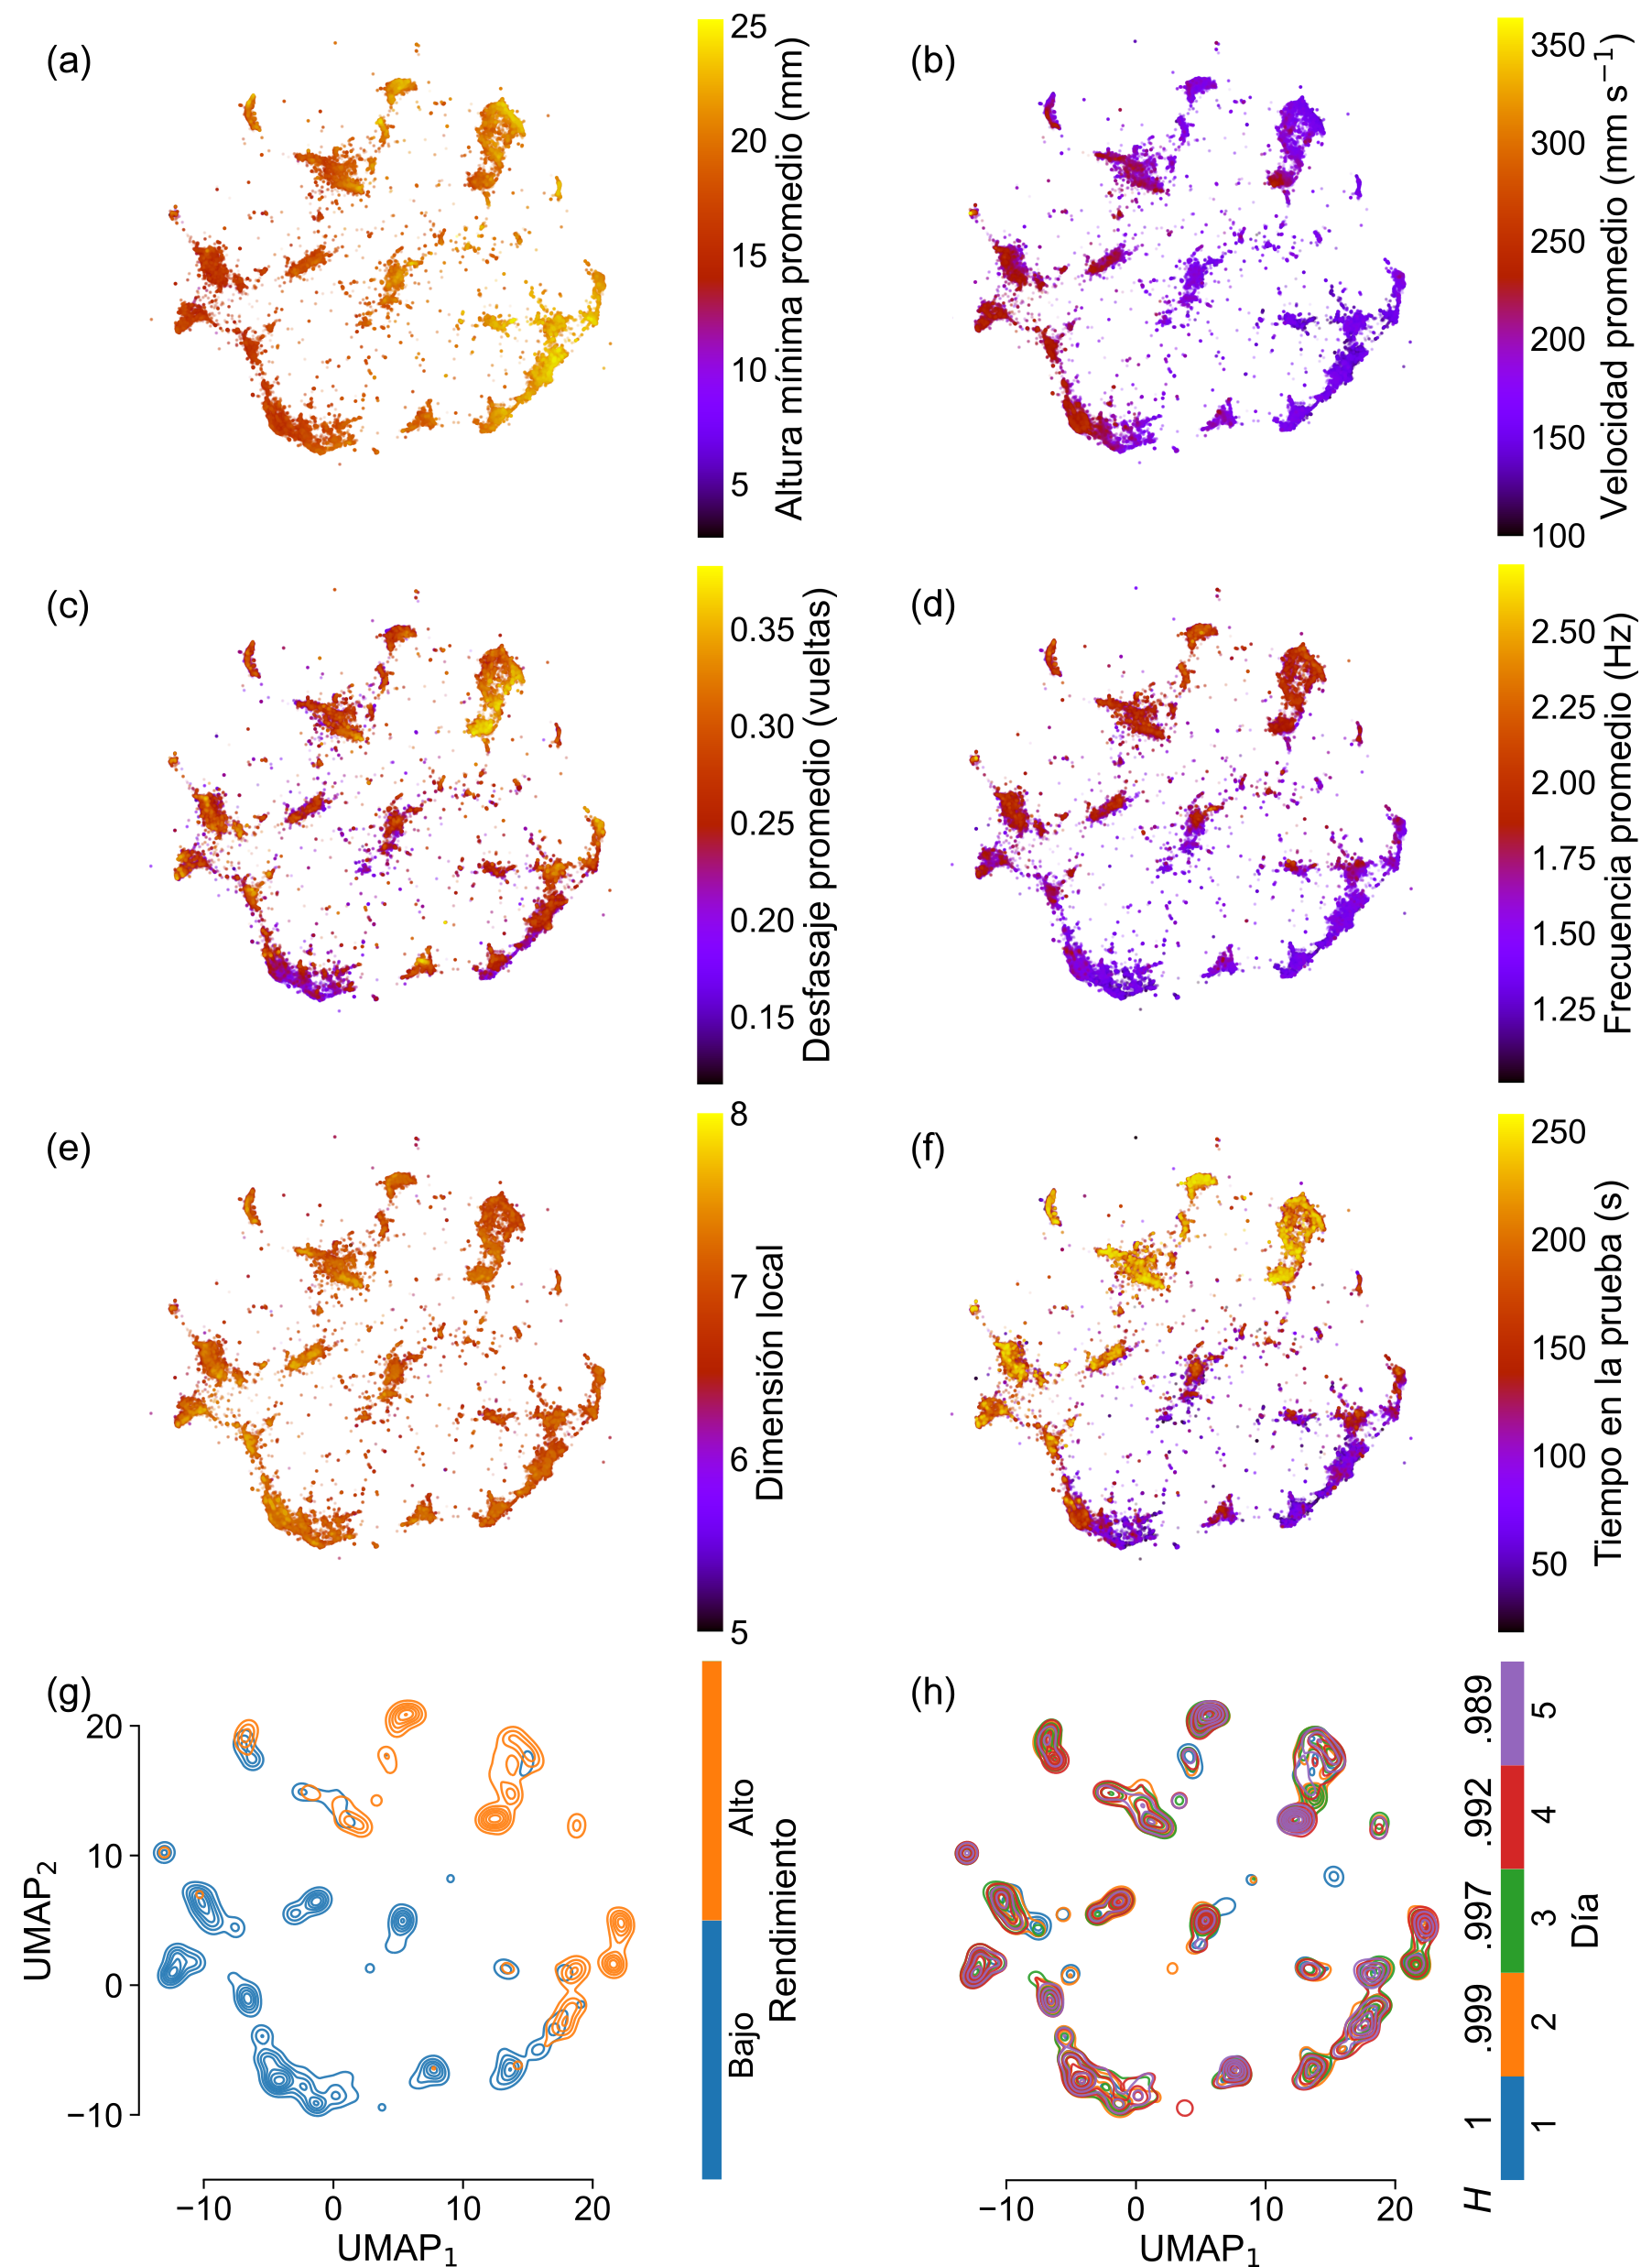
\includegraphics[width=0.9\linewidth]{figuras/capitulo4/umap_stp.png}
        \caption{\textbf{UMAP de las características de pasos y poses.} Valores promedio de algunas características de pasos: (a) altura mínima, (b) velocidad, (c) desfasaje y (d) frecuencia. (e) Dimensión local del mapa. La dimensión local es el número de componentes PCA que explican el 80\% de la varianza en el subconjunto de datos formado por los vecinos más cercanos de cada punto en el mapa. (f) Tiempo transcurrido en cada prueba rotarod. (g) Densidad de probabilidad  en el espacio UMAP, condicionada por grupo de rendimiento. (h) Densidad de probabilida condicionada por día de entrenamiento. La entropía $H$ de las distribuciones disminuye con los días de entrenamiento, tomando como valor de referencia a la entropía del día 1.}
        \label{fig:capitulo4_umap_stp}
    \end{figure}

    \clearpage

    \section{\textit{Labels} de comportamiento}\label{sec:apendice_labels}

    \begin{figure}[htbp]
        \centering
        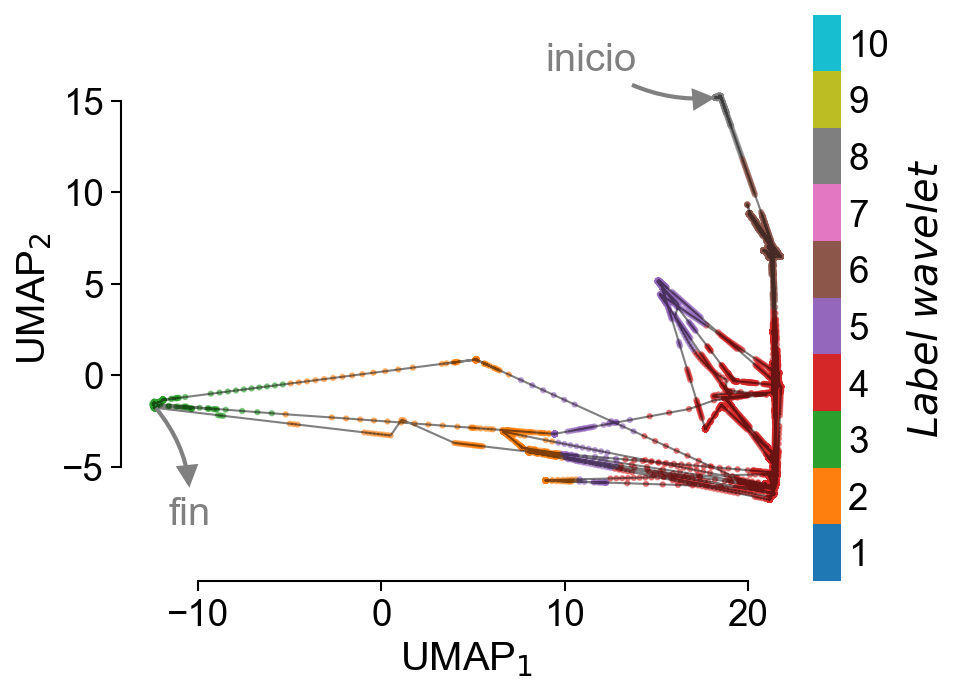
\includegraphics[width=0.7\linewidth]{figuras/capitulo4/label_serie_mapa_wav.png}
        \caption{\textbf{\textit{Labels} de comportamiento en el mapa UMAP \textit{wavelet}.}
            Serie temporal de \textit{labels}, vistos en el mapa UMAP \textit{wavelet}, durante la ejecución de una prueba rotarod (ídem \autoref{fig:capitulo2_posiciones})}
        \label{fig:capitulo4_label_serie_mapa_wav}
    \end{figure}

    \begin{figure}[htbp]
        \centering
        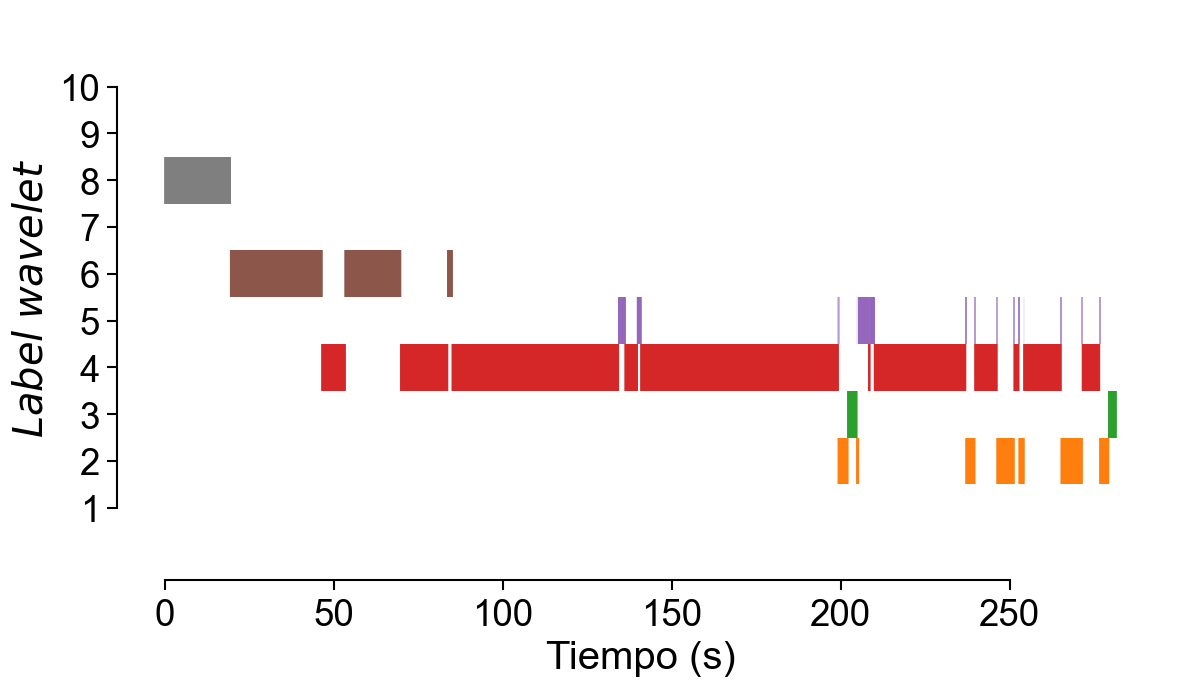
\includegraphics[width=0.7\linewidth]{figuras/capitulo4/label_secuencia_wav.png}
        \caption{\textbf{Secuencia de \textit{labels} \textit{wavelet}.}
            Secuencia de \textit{labels wavelet} durante la ejecución de una prueba rotarod (ídem \autoref{fig:capitulo2_posiciones})}
        \label{fig:capitulo4_label_secuencia_wav}
    \end{figure}

    \begin{figure}[htbp]
        \centering
        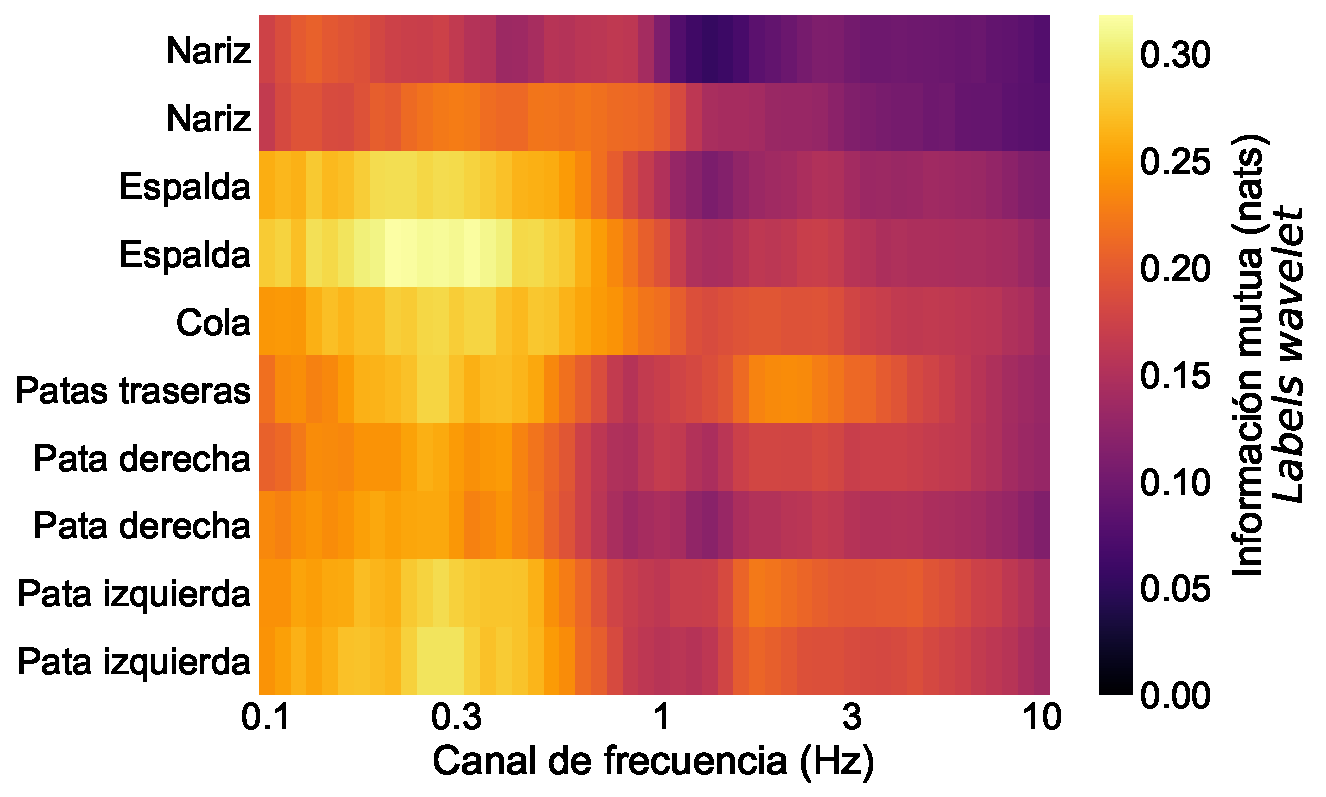
\includegraphics[width=0.7\linewidth]{figuras/capitulo4/mi_labels_wav.pdf}
        \caption{\textbf{Información mutua entre los \textit{labels} \textit{wavelets} y los espectros \textit{wavelet}.}}
        \label{fig:capitulo4_mi_labels_wav}
    \end{figure}

    \begin{figure}[htbp]
        \centering
        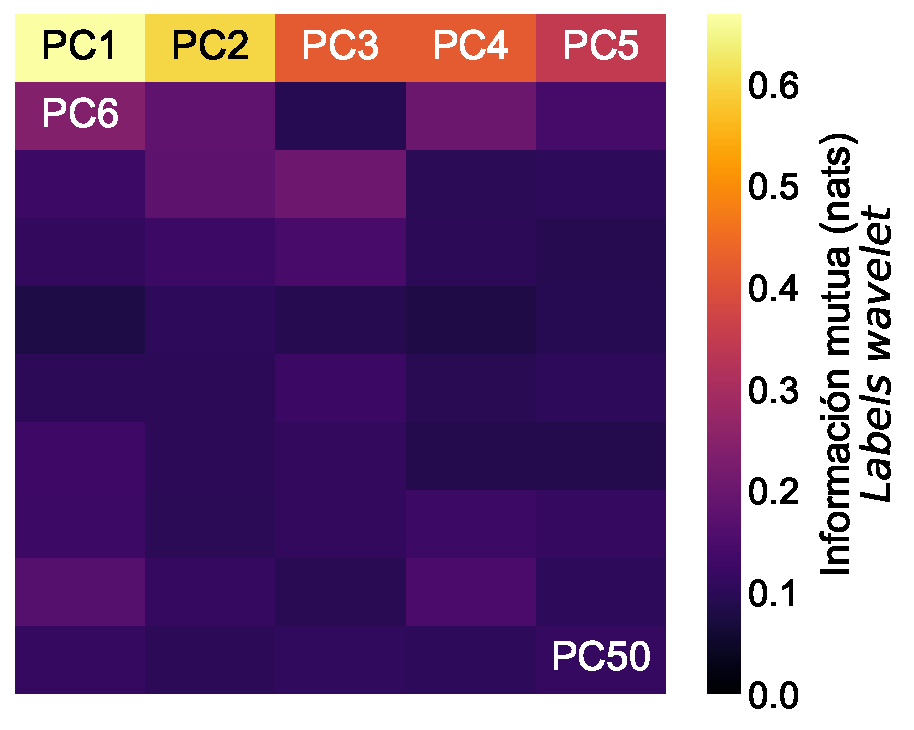
\includegraphics[width=0.7\linewidth]{figuras/capitulo4/mi_labels_pca.pdf}
        \caption{\textbf{Información mutua entre los \textit{labels} \textit{wavelets} y el PCA de los espectros \textit{wavelet}.}}
        \label{fig:capitulo4_mi_labels_pca}
    \end{figure}

    \begin{figure}[htbp]
        \centering
        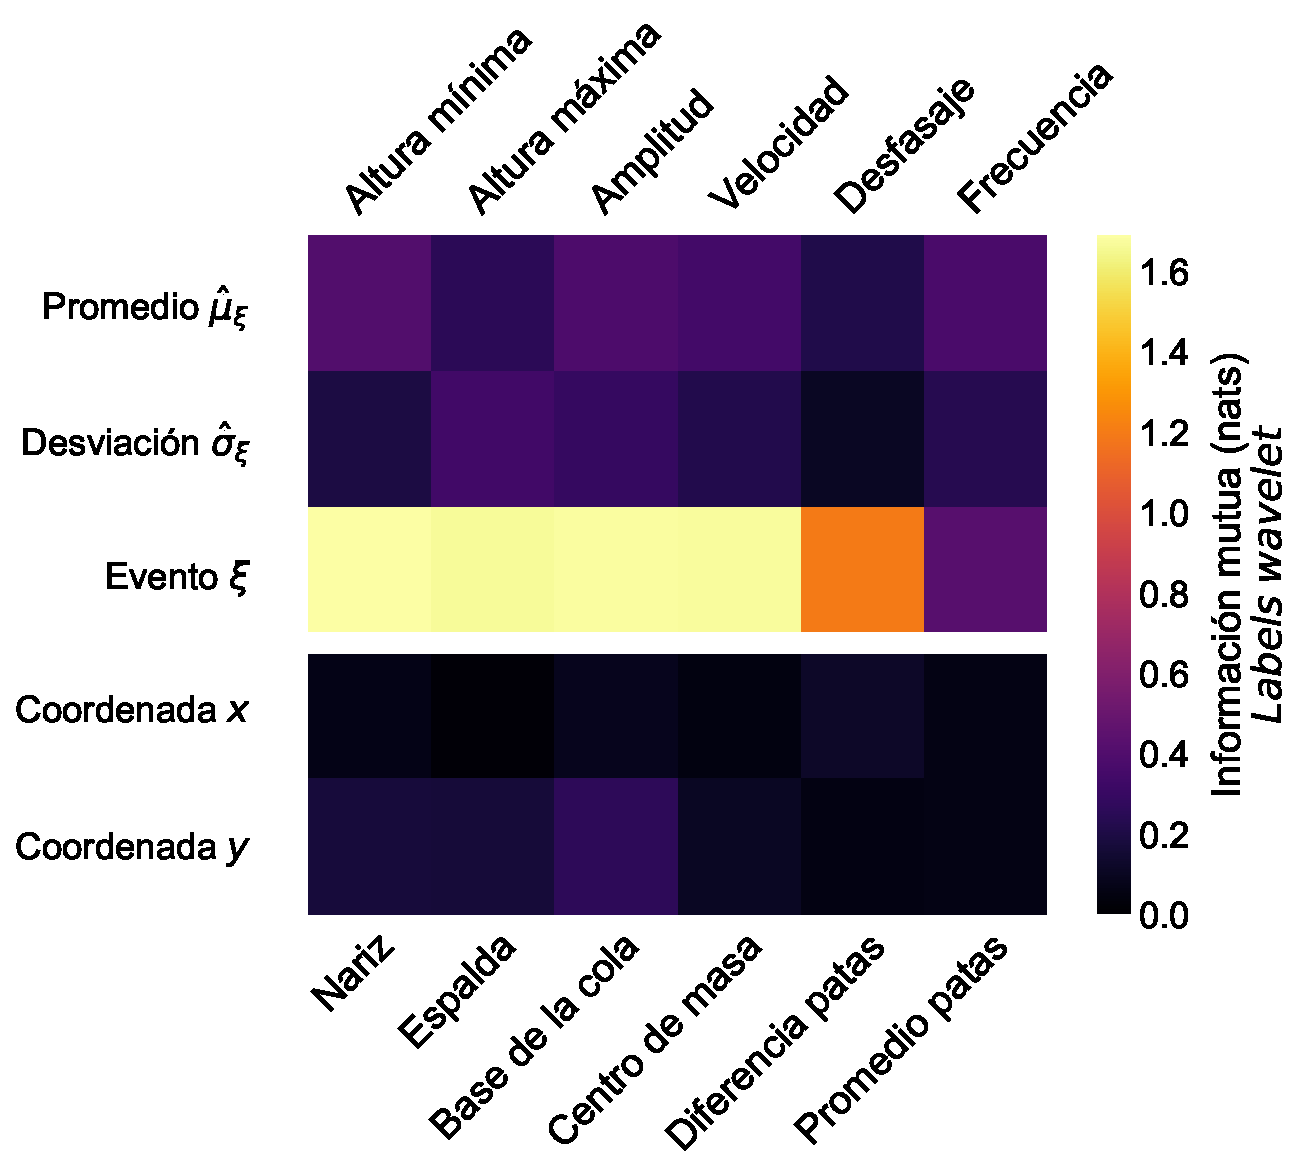
\includegraphics[width=0.7\linewidth]{figuras/capitulo4/mi_contra_labels_scaler_stp.pdf}
        \caption{\textbf{Información mutua entre los \textit{labels} \textit{wavelets} y las características de pasos y poses.}}
        \label{fig:capitulo4_mi_contra_labels_scaler_stp}
    \end{figure}

    \begin{figure}[htbp]
        \centering
        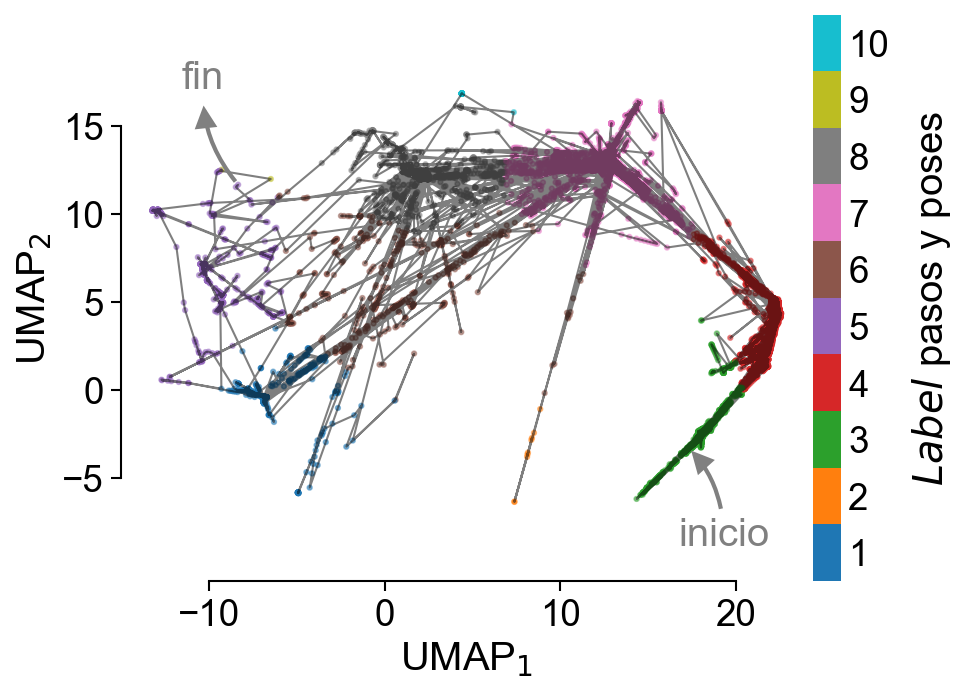
\includegraphics[width=0.7\linewidth]{figuras/capitulo4/label_serie_mapa_stp.png}
        \caption{\textbf{\textit{Labels} de comportamiento en el mapa UMAP de pasos y poses.}
            Serie temporal de \textit{labels}, vistos en el mapa UMAP de pasos y poses, durante la ejecución de una prueba rotarod (ídem \autoref{fig:capitulo2_posiciones})}
        \label{fig:capitulo4_label_serie_mapa_stp}
    \end{figure}

    \begin{figure}[htbp]
        \centering
        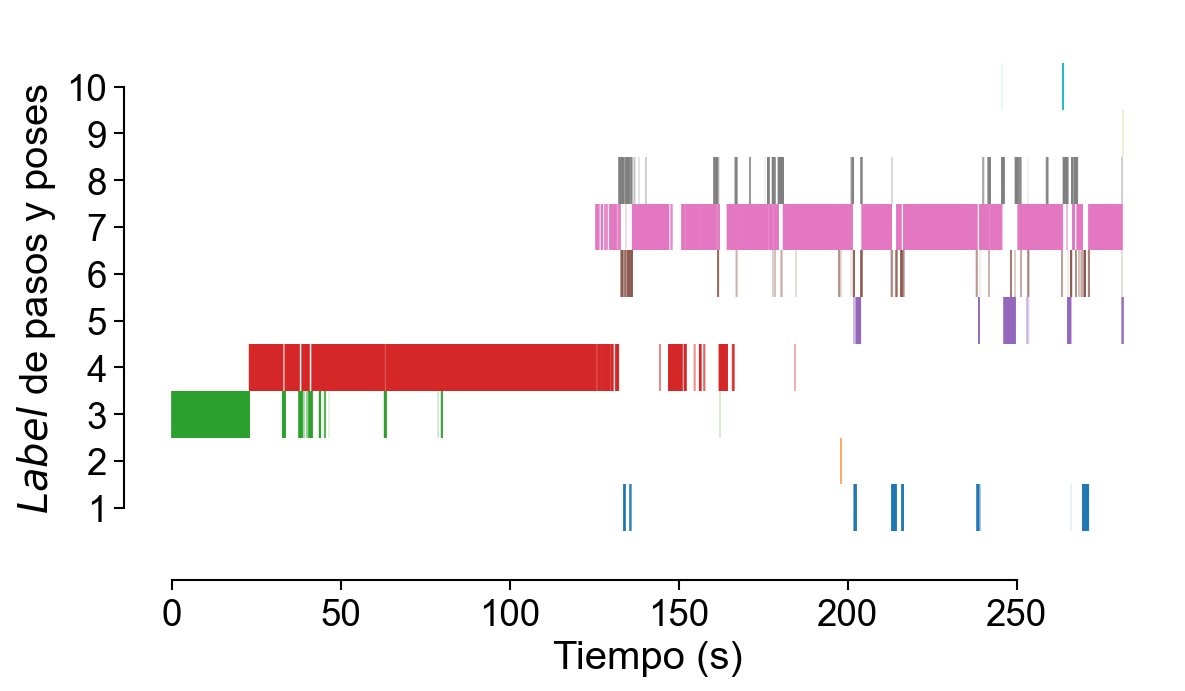
\includegraphics[width=0.7\linewidth]{figuras/capitulo4/label_secuencia_stp.png}
        \caption{\textbf{Secuencia de \textit{labels} de pasos y poses.}
            Secuencia de \textit{labels} de pasos y poses durante la ejecución de una prueba rotarod (ídem \autoref{fig:capitulo2_posiciones})}
        \label{fig:capitulo4_label_secuencia_stp}
    \end{figure}

    \begin{figure}[htbp]
        \centering
        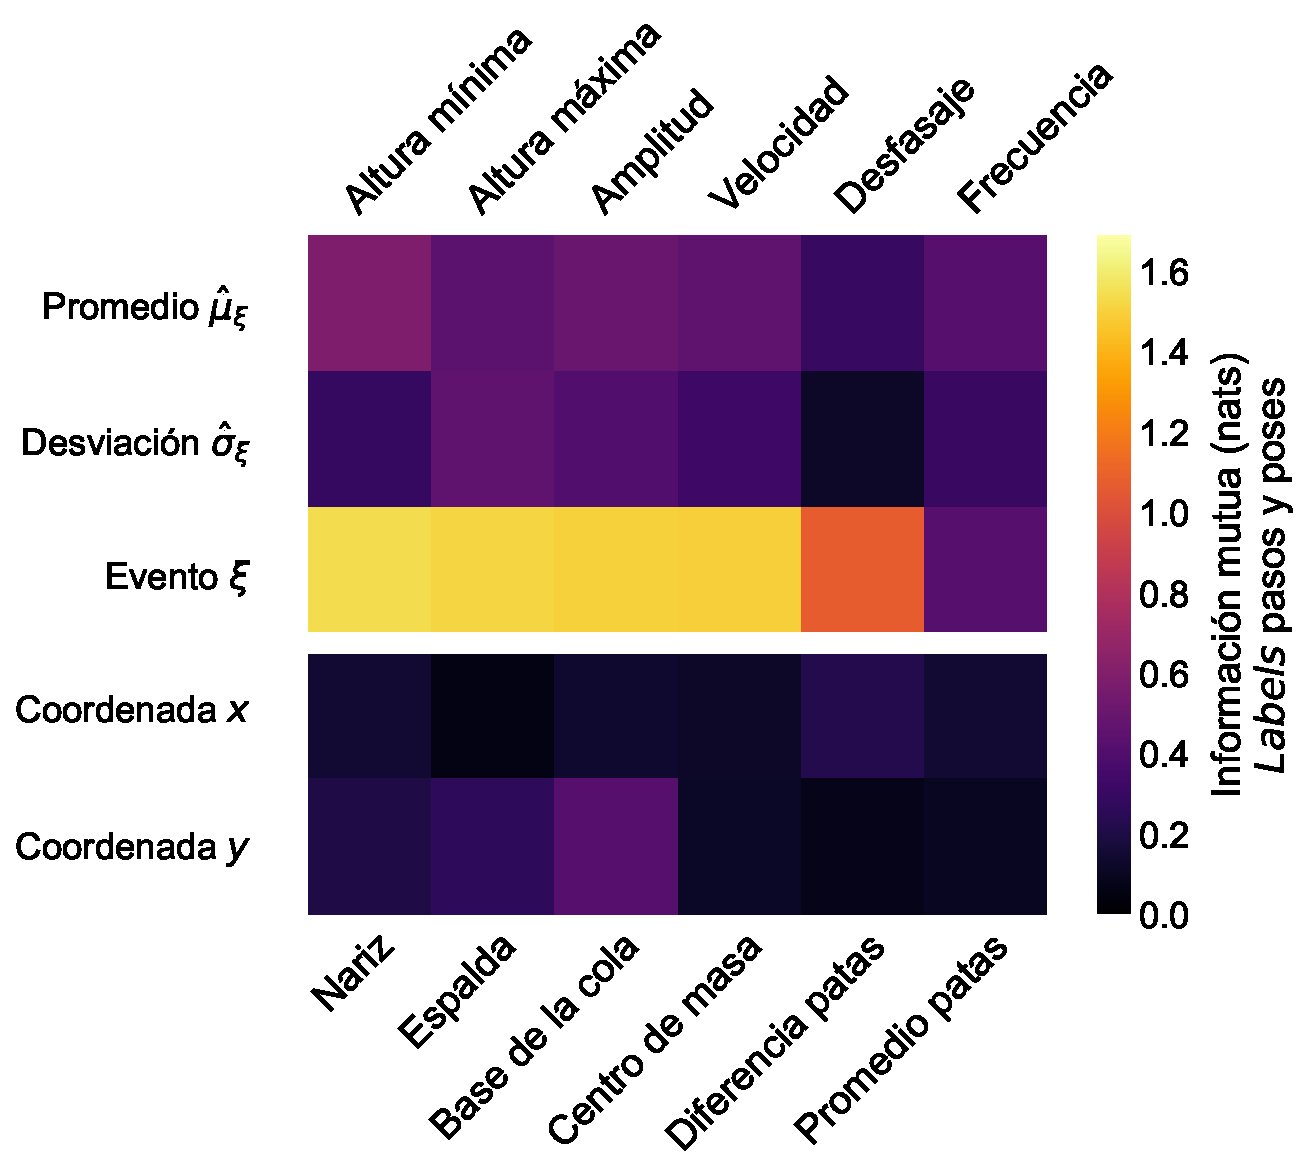
\includegraphics[width=0.7\linewidth]{figuras/capitulo4/mi_labels_scaler_stp.pdf}
        \caption{\textbf{Información mutua entre los \textit{labels} pasos y poses y las características de pasos y poses.}}
        \label{fig:capitulo4_mi_labels_scaler_stp}
    \end{figure}

    \begin{figure}[htbp]
        \centering
        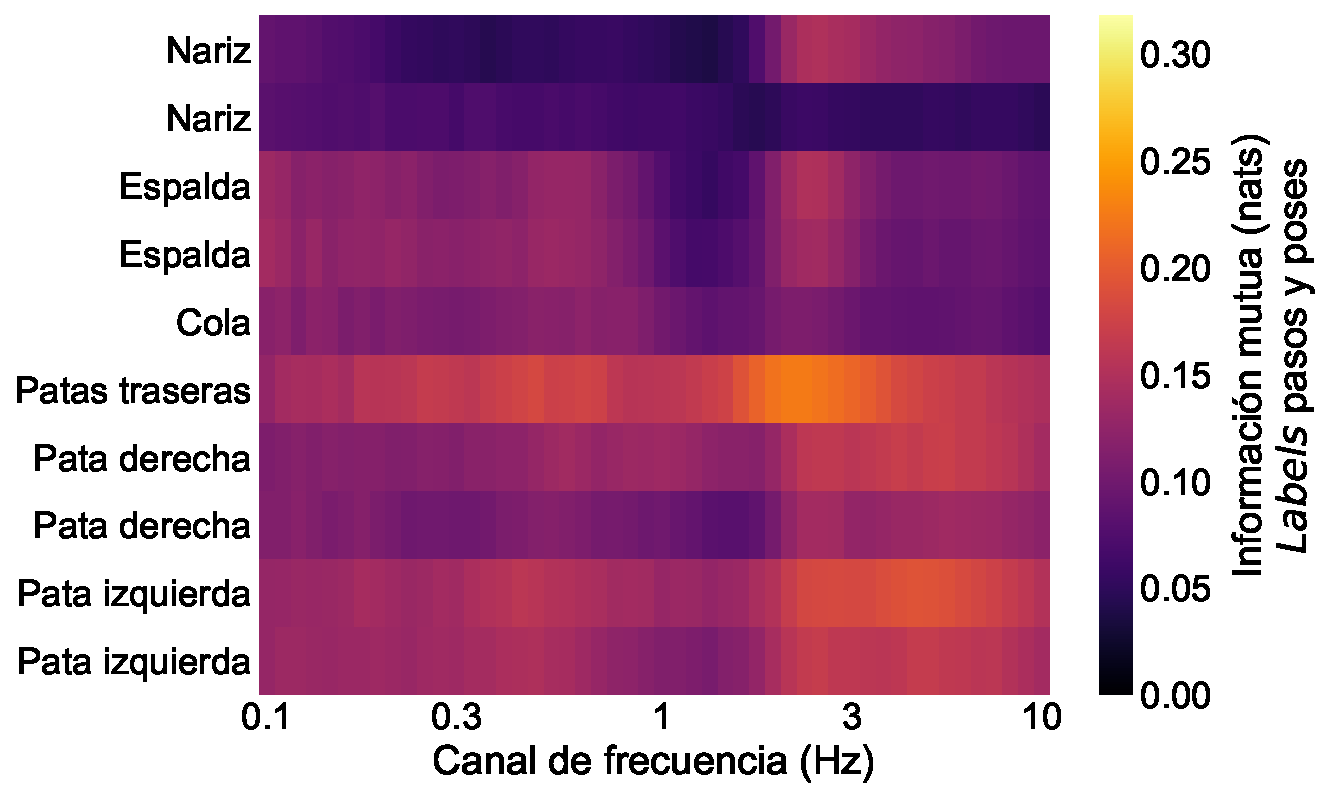
\includegraphics[width=0.7\linewidth]{figuras/capitulo4/mi_contra_labels_wav.pdf}
        \caption{\textbf{Información mutua entre los \textit{labels} pasos y poses y los espectros \textit{wavelet}.}}
        \label{fig:capitulo4_mi_contra_labels_wav}
    \end{figure}

    \begin{figure}[htbp]
        \centering
        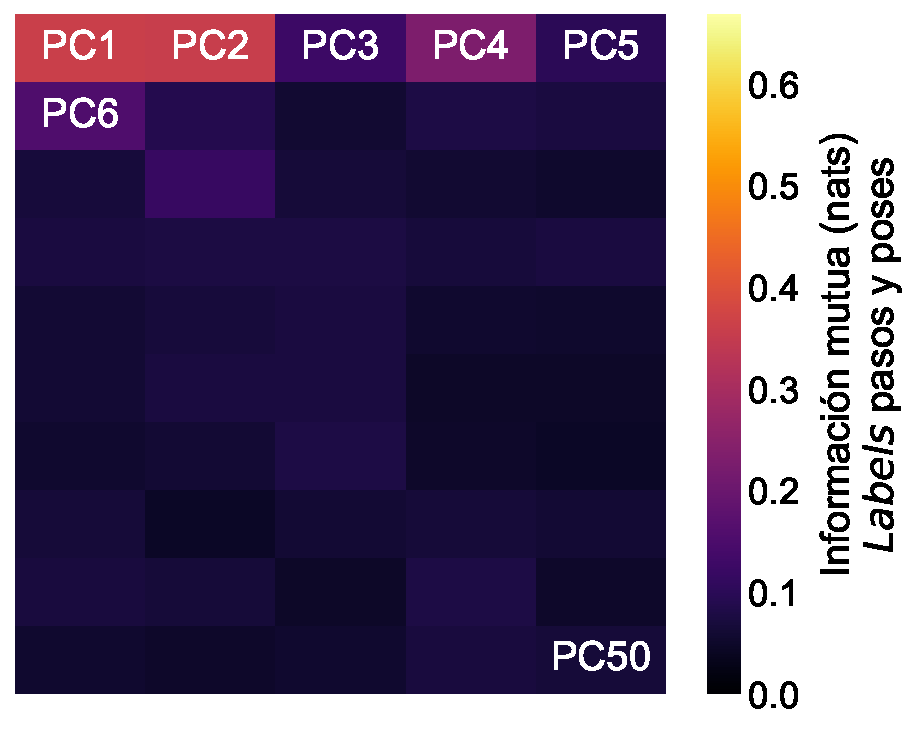
\includegraphics[width=0.7\linewidth]{figuras/capitulo4/mi_contra_labels_pca.pdf}
        \caption{\textbf{Información mutua entre los \textit{labels} pasos y poses y el PCA de los espectros \textit{wavelet}.}}
        \label{fig:capitulo4_mi_contra_labels_pca}
    \end{figure}

\end{appendix}